\documentclass[11pt]{book}
\usepackage{amsmath, amsthm, amssymb, bm, bbm}
\usepackage{amsfonts}
\usepackage{tikz}
\usepackage[utf8]{inputenc}
\usepackage[T1]{fontenc}
\usepackage{lmodern}

\usepackage{framed}
\definecolor{timberwolf}{rgb}{0.94, 0.94, 0.94}
\definecolor{azure}{rgb}{0.9, 0.95, 1.0}
\colorlet{shadedef}{timberwolf}
\colorlet{framedef}{timberwolf}
\colorlet{shadethm}{azure}
\colorlet{framethm}{azure}

\addtolength{\topmargin}{-1in}
\addtolength{\textwidth}{1in}
\addtolength{\evensidemargin}{-0.7in}
\addtolength{\textheight}{1.25in}

\newcommand{\norm}[1]{\left\lVert#1\right\rVert}
\newcommand{\inp}[2]{\langle #1,#2\rangle}
\newcommand{\vc}[1]{\textbf{\underline{#1}}}
\newcommand{\Ex}[0]{\vc{Ex}: }
\newcommand{\R}[1]{\mathbb{R}^{#1}}
\newcommand{\C}[1]{\mathbb{C}^{#1}}
\newcommand{\pf}[1]{\textbf{\underline{Proof}}: #1 $\;\;\blacksquare$}
\newcommand{\ub}[1]{\textbf{\underline{#1}}}
\newcommand{\OO}[0]{\mathcal{O}}
\newcommand{\TT}[0]{\mathcal{T}}
\newcommand{\CC}[0]{\mathcal{C}}
\newcommand{\FF}[0]{\mathcal{F}}
\newcommand{\MM}[0]{\mathcal{M}}
\newcommand{\LL}[0]{\mathcal{L}}
\newcommand{\HH}[0]{\mathcal{H}}
\newcommand{\Sm}[0]{\mathcal{S}}
\newcommand{\se}[0]{\subseteq}
\newcommand{\bint}[0]{\displaystyle\int}
\newcommand{\sif}[0]{\text{SIF}(S,\mu)}
\newcommand{\xsm}[0]{(X,\Sm,\mu)}
\newcommand{\xsmb}[1]{(X,\Sm,\mu,{#1})}
\newcommand{\muf}[0]{\mu_{\varphi}}
\makeindex

\newenvironment{prop}{%
  \def\FrameCommand{\fboxrule=\FrameRule\fboxsep=\FrameSep \fcolorbox{framethm}{shadethm}}%
  \MakeFramed {\FrameRestore}\noindent\textbf{\underline{Proposition}}:}%
{\endMakeFramed}

\newenvironment{lemma}{%
  \def\FrameCommand{\fboxrule=\FrameRule\fboxsep=\FrameSep \fcolorbox{framethm}{shadethm}}%
  \MakeFramed {\FrameRestore}\noindent\textbf{\underline{Lemma}}:}%
{\endMakeFramed}

\newenvironment{thm}{%
  \def\FrameCommand{\fboxrule=\FrameRule\fboxsep=\FrameSep \fcolorbox{framethm}{shadethm}}%
  \MakeFramed {\FrameRestore}\noindent\textbf{\underline{Theorem}}:}%
{\endMakeFramed}

\newenvironment{cor}{%
  \def\FrameCommand{\fboxrule=\FrameRule\fboxsep=\FrameSep \fcolorbox{framethm}{shadethm}}%
  \MakeFramed {\FrameRestore}\noindent\textbf{\underline{Corollary}}:}%
{\endMakeFramed}

\newenvironment{defn}{%
  \def\FrameCommand{\fboxrule=\FrameRule\fboxsep=\FrameSep \fcolorbox{framedef}{shadedef}}%
  \MakeFramed {\FrameRestore}\noindent\textbf{\underline{Def}}:}%
{\endMakeFramed}

\newenvironment{frame*}{%
  \def\FrameCommand{\fboxrule=\FrameRule\fboxsep=\FrameSep \fcolorbox{framethm}{shadethm}}%
  \MakeFramed {\FrameRestore}}%
{\endMakeFramed}


\title{Math 202B: Topology and Analysis II Lecture Notes}
\author{Joseph Pagadora \\ Instructor: Marc Rieffel}
\date{Spring 2019}

\begin{document}
\maketitle

\tableofcontents

\chapter{Metric Spaces}
\section{Fundamentals}
\begin{defn}
Let $X$ be a set. A \vc{metric} on $X$ is a function $d:X\times X\rightarrow [0,\infty)$ that satisfies: 
\begin{enumerate}
\item[(a)] $d(x,y)=d(y,x)$ for any $x,y\in X$
\item[(b)] $d(x,y)\leq d(x,z)+d(z,y)$ for any $x,y,z\in X$
\item[(c)] $d(x,y)=0$ iff $x=y$
\end{enumerate}
If a function $d$ satisfies (a), (b) above, and $d(x,x)=0$ for all $x\in X,$ then $d$ is a \vc{semi-metric}.
\end{defn}

\Ex On $\C{n},$ the following are common metrics:
\begin{itemize}
\item $d_p(v,w)=\Big(\sum\limits_{j=1}^n |v_j-w_j|^p\Big)^{1/p}$ for $p\geq 1$
\item $d_{\infty}(v,w)=\sup\{|v_j-w_j|:1\leq j\leq n\}$
\end{itemize}
(Verify that these are metrics.) \\ \\
Fact: If $S\subseteq X,$ and $d$ is a metric on $X,$ then $d$ is a metric on $S.$ \\

\begin{defn} 
Let $V$ be a vector space over $\R{ }$ or $\C{ }.$ A \vc{norm} on $V$ is a function $\norm{\cdot}:V\rightarrow[0,\infty)$ such that:
\begin{enumerate}
\item[(a)] $\norm{cv}=|c|\cdot\norm{v}$ for $c\in \R{}$ or $\C{}$ and $v\in V$
\item[(b)] $\norm{v+w}\leq\norm{v}+\norm{w}$ for $v,w\in V$
\item[(c)] $\norm{v}=0$ implies $v=0$
\end{enumerate}
A function that satisfies only (a) and (b) above is called a \vc{seminorm}.
\end{defn}

\noindent Remark: Any norm $\norm{\cdot}$ on $X$ induces the metric $d(x,y):=\norm{x-y}.$ \\ \\ \\
\Ex Let $V$ be the space of continuous functions on $[0,1].$ Then  \\ $\norm{f}_{\infty}=\sup\{|f(x)|:x\in[0,1]\}$ is a norm on $V.$ \\
It can also be shown that $\norm{f}_p:=\Big(\int_0^1 |f(x)|^p\;dx\Big)^{1/p}$ is a norm on $V.$ \\

\begin{defn}
Let $(X,d_x)$ and $(Y,d_y)$ be metric spaces. A function $f:X\rightarrow Y$ is \vc{isometric} if $d_y(f(v),f(w))=d_x(v,w)$ for all $v,w\in X.$
\end{defn}
\begin{itemize}
\item Note that all isometries are injective.
\end{itemize}

\noindent\Ex If $S\subseteq X,$ and $f:S\rightarrow X$ is defined by $f(x)=x$ (inclusion), then $f$ is an isometry. \\ \\
If $f$ is onto, then $f$ is viewed as an isomorphism between $(X,d_x)$ and $(Y,d_y).$ $f^{-1}$ is also an isomorphism.
\begin{defn} 
A function $f:X\rightarrow Y$ is \vc{Lipschitz} if there is a constant $k\geq 0$ such that $d_y(f(x_1),f(x_2))\leq k\cdot d_x(x_1,x_2).$ The smallest such constant is the \vc{Lipschitz constant} for $f.$
\end{defn}

\begin{defn} 
$f:X\rightarrow Y$ is \vc{uniformly continuous} if for any $\epsilon>0,$ there exists $\delta>0$ such that $d_y(f(x_1),f(x_2))<\epsilon$ whenever $d_x(x_1,x_2)<\delta.$
\end{defn}
\begin{itemize}
\item It is easy to see that if $f$ is Lipschitz, then it is uniformly continuous.
\end{itemize}

\begin{defn} 
$f:X\rightarrow Y$ is \vc{continuous at $x_0$} if for any $\epsilon>0,$ there exists $\delta>0$ such that $d_y(f(x),f(x_0))<\epsilon$ whenever $d_x(x,x_0)<\delta.$ We say $f$ is \vc{continuous} if it is continuous at every $x\in X.$
\end{defn}

\begin{defn} 
A sequence $\{x_n\}$ in $X$ \vc{converges} to $x^*\in X$ if for any $\epsilon>0,$ there exists $N\in\mathbb{N}$ such that for all $n\geq N,$ we have $d(x_n,x^*)<\epsilon.$
\end{defn}

\begin{prop} 
A function $f:X\rightarrow Y$ is continuous iff $x_n\rightarrow x$ implies $f(x_n)\rightarrow f(x).$ \\ \\
\pf{\textit{Exercise.}}
\end{prop}

\begin{defn}
$S\subseteq X$ is \vc{dense} in $X$ if for any $x\in X$ and $\epsilon>0,$ there exists $s\in S$ such that $d(x,s)<\epsilon.$
\end{defn}

\begin{prop}
Let $S$ be dense in $X,$ and let $f:X\rightarrow Y$ and $g:X\rightarrow Y$ be continuous functions such that $f(s)=g(s)$ for all $s\in S.$ Then $f=g$ on $X.$ \\ \\
\pf{Let $x\in X\setminus S,$ and let $\epsilon>0.$ Then there exists $\delta>0$ and $s\in S$ such that $d(f(x),f(s))<\epsilon/2,$ and $d(g(x),g(s))<\epsilon/2$ for $d(x,s)<\delta,$ by continuity and density. Then 
$$d(f(x),g(x))\leq d(f(x),f(s))+d(g(s),g(x))<\epsilon/2+\epsilon/2=\epsilon,$$
since $f(s)=g(s).$ Thus $d(f(x),g(x))=0,$ so $f(x)=g(x).$}
\end{prop}

\begin{defn}
A sequence $\{x_n\}$ is \vc{Cauchy} if for any $\epsilon>0,$ there exists $N\in\mathbb{N}$ such that $n,m\geq N$ implies $d(x_n,x_m)<\epsilon.$ \\
A metric space in which every Cauchy sequence converges is \vc{complete}.
\end{defn}

\noindent\Ex Consider $(\mathbb{Q}, |\cdot|).$ We know there exists a Cauchy sequence converging to $\sqrt{2}\in\mathbb{R},$ but in this metric space, $\sqrt{2}$ is not an element, so this sequence does not converge, hence this metric space is not complete.

\section{Completion of a Metric Space}

\begin{prop}
If $f:X\rightarrow Y$ is uniformly continuous, and $\{x_n\}$ is Cauchy in $X,$ then $\{f(x_n)\}$ is Cauchy in $Y.$ \\ \\
\pf{\textit{Exercise.}}
\end{prop}

\begin{defn}
Let $(X,d)$ be a metric space. A complete metric space $(\overline{X},\overline{d}),$ together with an isometric function $f:X\rightarrow\overline{X}$ with dense range is a \vc{completion} of $(X,d).$
\end{defn}
\begin{itemize}
\item Remark: Completions are unique up to isomorphism.
\end{itemize}

\begin{prop}
If $((Y_1, d_1), f_1)$ and $((Y_2,d_2),f_2)$ are completions of $(X,d),$ then there exists an onto isometry (metric space isomorphism) $g:Y_1\rightarrow Y_2$ with $f_2=g\circ f_1.$ This can be visualized by the following commutative diagram: \\
\begin{center}
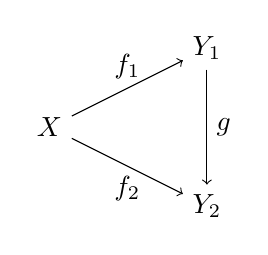
\begin{tikzpicture}
\node (a) at (0,0) {$X$};
\node (b) at (2,1) {$Y_1$};
\node (c) at (2,-1) {$Y_2$};
\draw[->] (a) -> (b) node[midway,above] {$f_1$};
\draw[->] (a) -> (c) node[midway,below] {$f_2$};
\draw[->] (b) -> (c) node[midway,right] {$g$};
\end{tikzpicture}
\end{center}
\end{prop}

\noindent Every metric space has a completion, and the proof will be constructive. The completion will be defined using equivalence classes of Cauchy sequences. We will need the following lemmas to support the construction.

\begin{frame*}
\noindent \ub{Lemma 1}: If $\{s_n\}$ and $\{t_n\}$ are Cauchy sequences in $X,$ then the sequence $\{d(s_n,t_n)\}$ in $\R{}$ converges. \\
\pf{\textit{Exercise. Hint:} $\{d(s_n,t_n)\}$ is a Cauchy sequence in a complete metric space.}
\end{frame*}

\begin{frame*}
\noindent \ub{Lemma 2}: Let $\text{Cau}(X)$ denote the set of all Cauchy sequences in $X.$ Then the relation $\{s_n\}\sim \{t_n\}$ iff $d(s_n,t_n)\rightarrow 0$ is an equivalence relation. \\ \\
\pf{Reflexivity and symmetry are trivial. Suppose $d(s_n,r_n)\rightarrow 0$ and $d(r_n,t_n)\rightarrow 0.$ Then $d(s_n,t_n)\leq d(s_n,r_n)+d(r_n,t_n)$ for all $n\in\mathbb{N}.$ The result follows immediately.}
\end{frame*}

\begin{frame*}
\noindent \ub{Lemma 3}: Let $\overline{X}$ be the set of all equivalence classes of $\text{Cau}(X)$ under the equivalence relation above. Then $\overline{d}:\overline{X}\rightarrow[0,\infty)$ defined by $\overline{d}(\{s_n\},\{t_n\}):=\lim\limits_{n\rightarrow\infty} d(s_n,t_n)$ is a metric on $\overline{X}.$ \\ \\
\pf{First, note that by Lemma 1, $\overline{d}$ is always defined. Since we are dealing with equivalence classes, we must show that $\overline{d}$ is also well-defined. Let $\xi,\eta\in\overline{X},$ and let $\{x_n\},\{s_n\}\in\xi,$ and $\{y_n\},\{t_n\}\in\eta.$ We have $\lim d(x_n,s_n)=\lim d(y_n,t_n)=0.$ Thus, \\ $d(s_n,t_n)\leq d(s_n,x_n)+d(x_n,y_n)+d(y_n,t_n).$ For any $\epsilon>0,$ we can find $N\in\mathbb{N}$ such that both $d(s_n,x_n)<\epsilon/2$ and $d(y_n,t_n)<\epsilon/2$ for $n\geq N.$ Then $|d(s_n,t_n)-d(x_n,y_n)|<\epsilon.$ It follows that $\overline{d}(\xi,\eta)=\lim d(x_n,y_n)=\lim d(s_n, t_n),$ so that $\overline{d}$ is indeed well-defined. \\  \\
Symmetry is trivial. The triangle inequality follows from the proof to Lemma 2. If $\overline{d}(\xi,\eta)=0,$ then for any $\{x_n\}\in\xi, \{y_n\}\in\eta,$ we have $\lim d(x_n,y_n)=0,$ so in particular, $\{y_n\}\in\xi,$ hence $\xi=\eta.$}
\end{frame*}

\begin{thm}
Let $(X,d_x)$ and $(Y,d_y)$ be metric spaces with $Y$ complete. If $S\subseteq X$ is dense, and $f:S\rightarrow Y$ is uniformly continuous, then there exists a unique continuous extension $\overline{f}:X\rightarrow Y$ of $f.$ In fact, $\overline{f}$ is uniformly continuous. \\ \\
\pf{(Existence only) For $x\in X,$ choose a Cauchy sequence $\{s_n\}$ in $S$ converging to $x.$ Then $\{f(s_n)\}$ is Cauchy in $Y,$ so it converges to a point $p\in Y.$ Set $\overline{f}(x):=p.$ We show that $\overline{f}$ is well-defined. Indeed, if $\{t_n\}\in\text{Cau}(S)$ and converges to $x,$ then we have $\lim d_x(s_n,t_n)=0,$ implying that $\lim d_y(f(s_n),f(t_n))=0.$ Therefore $\lim d_y(f(t_n),p)=0,$ so $\{f(t_n)\}$ converges to $p$ also. It remains to show continuity, which is left as an exercise.}
\end{thm}

\begin{thm}
Every metric space $(X,d)$ has a completion. \\ \\
\pf{As in Lemma 3, $(\overline{X},\overline{d})$ is a completion of $(X,d).$ We embed $X$ in $\overline{X}$ by the isometry $\iota:X\rightarrow\overline{X}$ defined by $\iota(x):= [\{x,x,x,...\}],$ where $[\cdot]$ denotes the corresponding equivalence class. Note that $\overline{d}\Big|_X=d,$ i.e., $\overline{d}(\iota(x),\iota(y))=d(x,y).$\\ It remains to show that $\overline{d}$ has dense range, and that $(\overline{X},\overline{d})$ is complete.
\begin{itemize}
\item Let $\xi\in\overline{X}, \epsilon>0, \{x_n\}\in\xi.$ There exists $N\in\mathbb{N}$ such that $n,m\geq N$ implies $d(x_n,x_m)<\epsilon.$ Then $\overline{d}(\iota(x_N),\xi)=\lim\limits_{n\rightarrow\infty} d(x_N,x_n)<\epsilon.$ Therefore $\overline{d}$ has dense range by considering $\iota(x_N).$
\item Let $\{\xi_n\}$ be a Cauchy sequence in $\overline{X}.$ For each $m\in\mathbb{N},$ pick $x_m\in X$ such that $\overline{d}(\iota(x_m),\xi_m)<1/m.$ Then $\{x_m\}$ is a Cauchy sequence, and it follows that $\{\xi_m\}$ converges to the equivalence class of $\{x_m\}.$
\end{itemize}}
\end{thm}

\noindent Remark on functions:\\
Denote $C([0,1])$ the space of continuous functions on $[0,1].$ Consider the metric space $C([0,1])$ induced by the norms $\norm{\cdot}_{\infty}$ or $\norm{\cdot}_p.$ This space is not complete. It is easy to come up with a sequence of continuous functions converging under these norms to a function that is not continuous. \\

\noindent Vector Space Remark: \\
Let $V$ be a vector space with norm $\norm{\cdot}.$ Consider $V^{\infty},$ the space of all sequences of elements in $V.$ This is also a vector space. It can be shown that $\text{Cau}(V)$ is a subspace of $V^{\infty}.$ \\
Now let $\mathcal{N}(V)$ denote the set of all Cauchy sequences in $V$ converging to $0.$ Then $\mathcal{N}(V)$ is a subspace of $\text{Cau}(V).$ If $\{v_n\}$ and $\{w_n\}$ are equivalent Cauchy sequences, then \\ $\norm{v_n-w_m}\rightarrow 0,$ so $\{v_n-w_n\}\in\mathcal{N}(V).$ Thus $\overline{V}$ is in fact the quotient space $\text{Cau}(V)/\mathcal{N}(V).$ \\ \\
Fact: Any two norms $\norm{\cdot}_1,\norm{\cdot}_2$ on a finite dimensional vector space are \ub{equivalent}, meaning that there are constants $c,C>0$ such that $c\norm{x}_1\leq\norm{x}_2\leq C\norm{x}_1$ for all $x.$ If a function is continuous with respect to a particular norm, then it is easily seen that it is continuous with respect to any equivalent norm.

\section{Openness}

\begin{defn}
If $(X,d)$ is a metric space, the \ub{open ball} of radius $r$ around $x$ is \\ $B_r(x):=\{y\in X: d(x,y)<r\}.$
\end{defn}

\begin{defn}
We can rephrase continuity as $f:X\rightarrow Y$ is continuous at $x_0$ if for any $\epsilon>0,$ there exists $\delta>0$ such that $f\Big(B_{\delta}(x_0)\Big)\subseteq B_{\epsilon}(f(x_0)).$
\end{defn}

\noindent
If $y\in B_{\epsilon}(f(x_0))$ and $y=f(x)$ for some $x\in X,$ let $\epsilon'=\epsilon-d(y,f(x_0))>0.$ Then $B_{\epsilon'}(y)\subseteq B_{\epsilon}(f(x_0)),$ so there exists $\delta'>0$ such that $f\Big(B_{\delta'}(x)\Big)\subseteq B_{\epsilon}(f(x_0)).$ \\
If $x_1\in f^{-1}\Big(B_{\epsilon}(f(x))\Big),$ there is an open ball $B_{\delta'}(x)$ such that $B_{\delta'}(x_1)\subseteq f^{-1}\Big(B_{\epsilon}(f(x))\Big).$ Thus $f^{-1}\Big(B_{\epsilon}(f(x))\Big)$ is a union of open balls in $X.$ Similarly, $f^{-1}(B_{\epsilon}(y))$ is a union of open balls in $X.$

\begin{defn}
A subset $\mathcal{O}\subseteq X$ (where $X$ is a metric space) is \ub{open} if it is a union of open balls in $X.$
\end{defn}

By the arguments above, it can be shown that $f:X\rightarrow Y$ is continuous iff for any open ball $B_{\epsilon}(y)\subseteq Y,$ we have that $f^{-1}(B_{\epsilon}(y))$ is open in $X.$ \\

\noindent Set theoretic facts:\\
Let $f:X\rightarrow Y$ be a function, and let $\{A_{\alpha}\}$ be a family of subsets of $X.$ Then:
\begin{itemize}
\item $f^{-1}\Big(\bigcup_{\alpha} A_{\alpha}\Big) = \bigcup_{\alpha} f^{-1}(A_{\alpha})$
\item $f^{-1}\Big(\bigcap_{\alpha} A_{\alpha}\Big) = \bigcap_{\alpha} f^{-1}(A_{\alpha})$
\item $f^{-1}\Big(A_1\setminus A_2) = f^{-1}(A_1)\setminus f^{-1}(A_2)$
\item $f\Big(\bigcup_{\alpha} A_{\alpha}\Big) = \bigcup_{\alpha} f(A_{\alpha})$
\item $f\Big(\bigcap_{\alpha} A_{\alpha}\Big) \subseteq \bigcap_{\alpha} f(A_{\alpha})$
\item $f(A_1\setminus A_2)\supseteq f(A_1)\setminus f(A_2)$
\end{itemize}

\noindent Let $\mathcal{O}\subseteq Y$ be open. Then $f^{-1}(\mathcal{O})=f^{-1}\Big(\bigcup\limits_{U\subseteq\mathcal{O}, U\text{ open ball}} U\Big)=\bigcup\limits_{U\subseteq\mathcal{O}, U\text{ open ball}} f^{-1}(U).$ \\ Thus, if $f:X\rightarrow Y$ is continuous, and $\mathcal{O}$ is open in $Y,$ then $f^{-1}(\mathcal{O})$ is open in $X.$
\begin{thm}
If $(X,d)$ is a metric space, and $\tau_d$ is the collection of all open sets, then:
\begin{enumerate}
\item[(1)] If $\{\mathcal{O}_{\alpha}\}$ is an arbitrary collection of subsets in $\tau_d,$ then $\bigcup_{\alpha}\mathcal{O}_{\alpha}$ is open.
\item[(2)] If $\mathcal{O}_1,\hdots,\mathcal{O}_n$ is a finite collection of subsets in $\tau_d,$ then $\bigcap\limits_{j=1}^n \mathcal{O}_j$ is open.
\item[(3)] $X\in\tau_d$ ($X$ is open)
\end{enumerate}
\pf{
  \begin{enumerate}
  \item[(1)] Trivial
  \item[(2)] Let $x\in \bigcap\limits_{j=1}^n \mathcal{O}_j.$ For each $j,$ there exists $\delta_j>0$ such that $B_{\delta_j}(x)\subseteq\mathcal{O}_j.$ Let \\ $\delta=\min\{\delta_j:1\leq j\leq n\}.$ Then $B_{\delta}(x)\subseteq\mathcal{O}_j$ for each $j.$ This yields the desired result.
  \item[(3)] Let $\epsilon>0.$ Then $X=\bigcup\limits_{x\in X} B_{\epsilon}(x).$ The result follows from (1).
  \end{enumerate}
}
\end{thm}
\noindent By convention, $\varnothing\in\tau_d$ ($\varnothing$ is open).
\chapter{$L^p$ Spaces}
\begin{defn}
Let $\xsm$ be a measure space, and let $0<p<\infty.$ Let $B$ be a Banach space, and let $f:X\rightarrow B$ be measurable. Then $f$ is \ub{$p$-integrable}, denoted $f\in \mathcal{L}^p(X,\mathcal{S},\mu, B),$ if the map $x\mapsto\norm{f(x)}^p$ is in $\mathcal{L}^1(X,\mathcal{S},\mu,\R{}).$ 
\end{defn}

Let $L^p$ denote the equivalence class of functions in $\mathcal{L}^p$ equal a.e. For now, we write $f\in L^p$ as any function in $\mathcal{L}^p$ equal a.e. to $f.$

\begin{prop}
$L^p\xsmb{B}$ is a vector space for pointwise operations. \\
\pf{Let $f,g\in L^p.$ Then 
$$\norm{f(x)+g(x)}^p\leq(2\cdot\max\{\norm{f(x)},\norm{g(x)}\})^p\leq 2^p(\norm{f(x)}^p+\norm{g(x)}^p)<\infty,$$
so $f+g\in L^p.$ It is obvious that for $c\in\R{},$ $cf\in L^p.$}
\end{prop}

For $f\in L^p,$ for now let us write $\norm{f}_p=\Big(\int\norm{f(x)}^p\;d\mu(x)\Big)^{1/p}.$ $\norm{\cdot}_p$ is not in general a norm. However, we will show that it is a norm for $p\geq 1.$

\begin{lemma}
If $p,q\in(1,\infty),$ and $p^{-1}+q^{-1}=1,$ and if $r>0,\; s>0,$ then $rs\leq\frac{r^p}{p}+\frac{s^q}{q}.$ \\
\pf{
	Since log is concave, we have
	$$\log\Big(\frac{1}{p}\cdot r^p+\frac{1}{q}\cdot s^q\Big)\geq\frac{1}{p}\log(r^p)+\frac{1}{q}\log(s^q)=\log(r)+\log(s)=\log(rs).$$
}
\end{lemma}

\begin{frame*}
\noindent\ub{Holder's Inequality}: If $p,q\in(1,\infty)$ and $p^{-1}+q^{-1}=1,$ and if $f\in L^p,\; g\in L^q,$ then $\int\norm{fg}\;d\mu\leq\norm{f}_p\norm{g}_q.$ \\
\pf{
	From the lemma, we have
	$$\frac{\norm{f(x)}}{\norm{f}_p}\cdot\frac{\norm{g(x)}}{\norm{g}_q}\leq\frac{\norm{f(x)}^p}{p\norm{f}_p^p}+\frac{\norm{g(x)}^q}{q\norm{g}_q^q}.$$
	Integrating, we get
	$$\int\frac{\norm{f(x)}}{\norm{f}_p}\cdot\frac{\norm{g(x)}}{\norm{g}_q}\;d\mu(x)\leq\frac{1}{p\norm{f}_p^p}\int\norm{f}^p\;d\mu+\frac{1}{q\norm{g}_q^q}\int\norm{g}^q\;d\mu=\frac{1}{p}+\frac{1}{q}=1.$$
}
\end{frame*}

For $g\in L^q,$ we can define $\varphi_g$ by $\varphi_g(f)=\int f(x)g(x)\;d\mu(x)$ for $f\in L^p.$ Then $\varphi_g$ is a linear functional, so its operator norm is $\norm{\varphi_g}\leq\norm{g}_q.$

\begin{prop}
For any $f\in L^p,$ there is $g\in L^q$, $\norm{g}_q=1,$ such that $\varphi_g(f)=\norm{f}_p.$ \\
\pf{
	Observe that $|f(x)|^p=(|f(x)|^{p/q})^q,$ so the map $x\mapsto |f(x)|^{p/q}\in L^q.$ It suffices to assume $\norm{f}_p=1.$ \\
	Let 
	$$u(x)=\begin{cases}
		0,\text{ if } f(x)=0,\\
		\frac{f(x)}{|f(x)|},\text{ if } f(x)\neq 0
	\end{cases}$$
	Then
	$$|u(x)|=\begin{cases}
		0,\text{ if } f(x)=0,\\
		1,\text{ if } f(x)\neq 0
	\end{cases}$$
	Let $g(x)=\overline{u(x)}|f(x)|^{p/q}$ so that $g\in L^q.$ Then
	$$\norm{g}_q=\Big(\int (|f(x)^{p/q})^q\Big)^{1/q}=\norm{f}_p^{p/q}=1,$$
	and
	$$\varphi_g(f)=\int\overline{u(x)}|f(x)|^{p/q} f(x)\;d\mu(x)=\int\overline{u(x)}|f(x)|^{p/q}u(x)|f(x)|\;d\mu(x)=$$
	$$=\int|f(x)|^{1+p/q}\;d\mu(x)=1=\norm{f}_p^p.$$
}
\end{prop}

\begin{frame*}
\noindent\ub{Minkowski's Inequality}: For $f,g\in L^p,$ we have $\norm{f+g}_p\leq\norm{f}_p+\norm{g}_p.$ \\
\pf{
	$$\norm{f+g}_p^p=\int|f(x)+g(x)|^p\;d\mu(x).$$
	By the previous proposition, there is $h\in L^q,$ where $h\geq 0,$ $\norm{h}_q=1,$ and 
	$$\norm{f+g}_p=\int|f+g|h\;d\mu\leq\int\Big(|f|+|g|\Big)h\;d\mu=\int|f|h\;d\mu+\int|g|h\;d\mu\leq$$
	$$\leq\norm{f}_p\norm{h}_q+\norm{g}_p\norm{h}_q=\norm{f}_p+\norm{g}_p.$$
}
\end{frame*}

\begin{thm}
$L^p(X,\Sm,\mu,B)$ is complete. \\
\pf{
	Let $\{f_n\}$ be a Cauchy sequence for the $p$-norm. We claim that $\{f_n\}$ is Cauchy in measure. For $m,n\in\mathbb{N},$ and $\epsilon>0,$ define
	$$E_{m,n}^{\epsilon}:=\{x:\norm{f_m(x)-f_n(x)}\geq\epsilon\}.$$
	For any $\epsilon>0,$ we have $\frac{1}{\epsilon}\chi_{E_{m,n}^{\epsilon}}(x)\leq\norm{f_m(x)-f_n(x)},$ so
	$$\frac{1}{\epsilon^p}\mu(E_{m,n}^{\epsilon})=\int\Big(\chi_{E_{m,n}^{\epsilon}}\Big)^p\;d\mu\leq\int\norm{f_m(x)-f_n(x)}^p\;d\mu(x)=\norm{f_m-f_n}_p^p\rightarrow 0$$
	as $m,n\rightarrow\infty.$ By the Riesz-Weyl Theorem, there is a subsequence that converges to some function $f$ a.e. Thus, we can assume without loss of generality that $f_n\rightarrow f$ a.e. \\
	For fixed $m,$ we have $|f_n(x)-f_m(x)|^p\rightarrow|f(x)-f_m(x)|^p$ as $n\rightarrow\infty,$ and by Fatou's Lemma, we have
	$$\int |f-f_m|^p\;d\mu\leq\lim\inf_{n\rightarrow\infty}\int|f_n-f_m|^p\;d\mu.$$
	For fixed $m,$ given $\epsilon>0,$ there is $N$ such that for $m,n\geq N,$
	$$\norm{f_m-f_n}_p<\epsilon^{1/p},\text{ i.e., } \int|f_n-f_m|^p\;d\mu<\epsilon.$$
	Therefore $\norm{f-f_n}_p^p<\epsilon,$ and thus $f_n\rightarrow f$ in the $p$-norm.
}
\end{thm}
\chapter{Compactness}

\section{Fundamentals}

\begin{defn}
\begin{itemize}
\item Let $X$ be a set, and let $\CC$ be a collection of subsets of $X.$ We say $\CC$ \ub{covers} $X$ if $\bigcup\limits_{A\in\CC}A=X.$
\item If $\CC$ is a cover of $X,$ and $\mathcal{D}\subseteq\CC$ is also a cover of $X,$ then $\mathcal{D}$ is a \ub{subcover} of $X.$
\item For a topological space $(X,\TT),$ an \ub{open cover} is a cover of $X$ that is contained in $\TT.$
\end{itemize}
\end{defn}

\begin{defn}
$(X,\TT)$ is \ub{compact} if every open cover of $X$ has a finite subcover.
\end{defn}

\begin{defn}
Let $\mathcal{F}$ be a collection of subsets of $X.$ Then $\mathcal{F}$ has the \ub{finite intersection property} if the intersection of any finite collection of sets in $\mathcal{F}$ is nonempty.
\end{defn}

\begin{prop}
$(X,\TT)$ is compact iff it has the property that whenever $\mathcal{F}$ is a collection of closed subsets of $X$ with the finite intersection property, then $\bigcap\limits_{A\in\mathcal{F}}A\neq\varnothing.$ \\ \\
\pf{\textit{Exercise}.}
\end{prop}

\begin{prop}
Let $(X,\TT)$ be a topological space. Then $A\subseteq X$ is compact for the relative topology iff for any open cover of $A,$ there is a finite subcover of $A.$ \\ \\
\pf{The open sets in the relative topology are exactly the sets of the form $A\cap\OO,$ where $\OO\in\TT.$}
\end{prop}

\begin{prop}
If $(X,\TT_x)$ is compact, and $(Y,\TT_y)$ is a topological space, and $f:X\rightarrow Y$ is continuous, then $f(X)$ is compact in $Y.$ \\ \\
\pf{Let $\CC\subseteq\TT_y$ be an open cover of $f(X).$ Then $\{f^{-1}(\OO)\}_{\OO\in\CC}$ is an open cover of $X,$ so there is a finite subcover $\{f^{-1}(\OO_1),...,f^{-1}(\OO_n)\}$ of $X.$ It follows that $f^{-1}(\OO_1)\cup\cdots\cup f^{-1}(\OO_n)=f^{-1}(\OO_1\cup\cdots\cup\OO_n)=X,$ so $\{\OO_1,\hdots,\OO_n\}$ is an open cover of $f(X).$}
\end{prop}

\begin{prop}
If $(X,\TT)$ is compact, and $A\subseteq X$ is closed, then $A$ is compact. \\ \\
\pf{
	Let $\CC$ be an open cover of $A.$ Since $A^c$ is open, $\CC\cup\{A^c\}$ covers $X,$ and since $(X,\TT)$ is compact, there is a finite subcover of $X,$ so clearly there is a finite subcover for $A.$
}
\end{prop}

\begin{prop}
If $(X,\TT)$ is Hausdorff, then any compact subset is closed. \\ \\
\pf{Let $A\subseteq X$ be compact, and let $x^*\not\in A.$ For any $y\in A,$ there are disjoint open sets $\OO_y,U_y$ such that $y\in\OO_y$ and $x^*\in U_y.$ Then $\{\OO_y:\;y\in A\}$ is an open cover of $A,$ so by compactness there is a finite subcover $\{\OO_{y_1},\hdots,\OO_{y_n}\}.$ Let $U=\bigcap\limits_{j=1}^n U_{y_j}.$ Then $U$ is open and covers $A^c$ and is also disjoint from $A.$ It follows that $U=A^c,$ and so $A$ is closed.
}
\end{prop}

\noindent Recall from standard real analysis the fact that in $\R{n},$ a subset is compact iff it is closed and bounded (Heine-Borel).

\begin{defn}
$(X,\TT)$ is \ub{regular} if for any closed set $A\subseteq X$ and any $x\not\in A,$ there are disjoint open sets $\OO, U$ such that $A\subseteq\OO$ and $x\in U.$
\end{defn}

\section{Tychonoff's Theorem}
We now develop an important compactness theorem of Tychonoff, which says that a product of compact spaces is compact in the product topology. In order to start, we need some set theory.

\begin{frame*}
\noindent \ub{Axiom of Choice}: Given any family of non-empty sets, there is a set containing an element from each of these sets.
\end{frame*}
\noindent We will see later that the axiom of choice is in fact equivalent to Tychonoff's Theorem.

\begin{defn}
A \ub{partially-ordered set} $P$ is a set with a partial order $\leq,$ which is a relation that satisfies
\begin{enumerate}
\item[(i)] $x\leq x$ for all $x\in P$
\item[(ii)] $x\leq y$ and $y\leq z$ implies $x\leq z$
\item[(iii)] If $x\leq y,$ and $y\leq x,$ then $x=y.$
\end{enumerate}
A \ub{totally/linearly-ordered} set satisfies the extra condition
\begin{enumerate}
\item[(iv)] For any $x,y\in P,$ either $x\leq y$ or $y\leq x.$
\end{enumerate}
\end{defn}

\noindent\Ex If $X$ is a set, consider its power set $\mathcal{P}(X).$ Then the relation $A\leq B$ iff $A\subseteq B$ is a partial order on $\mathcal{P}(X)$ but not a total order. \\
\Ex In the plane $\R{2},$ the relation $x\leq y$ iff $\norm{x}_2\leq\norm{y}_2$ is \textit{not} a partial order, since two points could have the same norm, but be unequal. \\
\Ex The usual relation $\leq$ on $\R{}$ is a total order.

\begin{defn}
\begin{itemize}
\item A \ub{chain} in $P$ is a totally-ordered subset of $P.$
\item A \ub{maximal element} in $P$ is an element $x\in P$ such that if $y\geq x,$ then $y=x.$
\item An \ub{upper bound} for a subset $A\subseteq P$ is an element $x\in P$ such that $y\leq x$ for all $y\in A.$
\item $P$ is \ub{inductively ordered} if every chain in $P$ has an upper bound.
\end{itemize}
\end{defn}

\begin{frame*}
\noindent \ub{Zorn's Lemma}: If $P$ is inductively ordered, then every chain $C$ has a maximal element $b$ for $C$ with $a\leq b$ for all $a\in C.$
\end{frame*}

\noindent Zorn's Lemma seems quite obscure, but it is incredibly practical in many important results in mathematics and particularly in analysis.

\begin{frame*}
\noindent \ub{Tychonoff's Theorem}: Let $\{(X_{\alpha},\TT_{\alpha})\}$ be a family of compact spaces indexed by $A.$ Then $X=\prod_{\alpha} X_{\alpha}$ with the product topology is compact. \\ \\
\pf{We will show compactness of $X$ through the finite intersection property. Let $\CC$ be a collection of closed subsets of $X$ with the finite intersection property. We wish to show that $\bigcap_{C\in\CC} C\neq\varnothing.$ \\ \\
	Let $\Theta=\{\mathcal{D}\subseteq \mathcal{P}(X): \CC\subseteq\mathcal{D},\; \mathcal{D}\text{ has finite intersection property}\}.$ \\
	Then $\Theta$ is partially ordered by set inclusion. To show that $\Theta$ is inductively ordered, let $\Phi\subseteq\Theta$ be a chain, and let $\mathcal{E}=\bigcup_{\mathcal{D}\in\Phi}\mathcal{D}.$ We show that $\mathcal{E}$ has the finite intersection property so that $\mathcal{E}\in\Theta$ and is thus an upper bound for $\Phi.$ \\
	Let $Z_1,\hdots,Z_n\in\mathcal{E}.$ Then there are $\mathcal{D}_1,\hdots,\mathcal{D}_n\in\Phi$ with $Z_j\in\mathcal{D}_j.$ Since $\Phi$ is totally ordered, one of the $\mathcal{D}_j$'s will be the largest, say, $\mathcal{D}_n,$ and each $\mathcal{D}_j\subseteq\mathcal{D}_n.$ Then $Z_1,\hdots,Z_n\in\mathcal{D}_n.$ But $\mathcal{D}_n$ has the finite intersection property, so $\bigcap\limits_{j=1}^n Z_j\neq\varnothing.$ Clearly $\CC\subseteq\mathcal{E},$ so $\mathcal{E}\in\Theta,$ and $\mathcal{E}$ is an upper bound for $\Phi.$ Thus $\Theta$ is inductively ordered, as desired. \\ \\
	By Zorn's Lemma, $\Theta$ contains a maximal element, say, $\mathcal{D}^*,$ which will have the following properties:
	\begin{itemize}
	\item If $Z_1,Z_2\in\mathcal{D}^*,$ then $Z_1\cap Z_2\in\mathcal{D}^*.$ \\ Indeed, for $Y_1,\hdots,Y_n\in\mathcal{D}^*,$ we have $(Z_1\cap Z_2)\cap(Y_1\cap\cdots\cap Y_n)\neq\varnothing.$ Therefore $\mathcal{D}^*\cup\{Z_1\cap Z_2\}$ has the finite intersection property. But by maximality of $\mathcal{D}^*,$ in fact $\mathcal{D}^*=\mathcal{D}^*\cup\{Z_1\cap Z_2\},$ therefore $Z_1\cap Z_2\in\mathcal{D}^*.$
	\item For $Y\subseteq X,$ if $Y\cap Z\neq\varnothing$ for all $Z\in\mathcal{D}^*,$ then $Y\in\mathcal{D}^*.$ \\ Indeed, for $Z_1,\hdots,Z_n\in Z,$ we have $Y\cap(Z_1\cap\cdots\cap Z_n)=\bigcap\limits_{j=1}^n (Y\cap Z_j)\neq\varnothing,$ and by maximality, $Y\in\mathcal{D}^*.$
	\end{itemize}
	For any $\mathcal{D}\in\Theta$ and for any $\alpha\in A,$ we claim that $\mathcal{F}_{\alpha}:=\{\pi_{\alpha}(Y):\;Y\in\mathcal{D}\}$ has the finite intersection property. By the finite intersection property of $\mathcal{D},$ for any $Z_1,\hdots,Z_n\in\mathcal{D},$ there exists $x\cap Z_1,\hdots\cap Z_n.$ Then $\pi_{\alpha}(x)\in\pi_{\alpha}(Z_1)\cap\cdots\cap\pi_{\alpha}(Z_n),$ thus $F_{\alpha}$ has the finite intersection property. It follows that $\Big\{\overline{\pi_{\alpha}(Z)}:\;Z\in\mathcal{D}\Big\}$ has the finite intersection property. This is a collection of closed subsets with the finite intersection property in $X_{\alpha},$ which is compact, so $\bigcap\limits_{Z\in\mathcal{D}}\overline{\pi_{\alpha}(Z)}\neq\varnothing.$ \\
	Apply this to each $\mathcal{D}\subseteq\mathcal{D}^*.$ For each $\alpha\in A,$ by the axiom of choice, pick $x_{\alpha}\in X_{\alpha}.$ \\
	Let $x=(x_{\alpha})\in\prod_{\alpha\in A} X_{\alpha}.$ We claim that $x\in\bigcap\limits_{C\in\CC}C.$ \\
	It suffices to show that if $\OO$ is an open set containing $x,$ then $\OO\cap C\neq\varnothing$ for all $C\in\CC.$ It further suffices to have $\OO$ be a basis element for the product topology. That is, suppose $x\in\OO=U_{\alpha_1}\times\cdots\times U_{\alpha_n}\times\prod\limits_{\alpha\neq \alpha_i\;\forall i} X_{\alpha}.$ \\
	Note that $x_{\alpha_j}\in U_{\alpha_j}$ for $j=1,\hdots,n.$ Then $x_{\alpha_j}\in\overline{\pi_{\alpha_j}(Z)}$ for all $Z\in\mathcal{D}^*,$ so $U_{\alpha_j}\cap\pi_{\alpha}(Z)\neq\varnothing$ for all $Z\in\mathcal{D}^*$ and for all $1\leq j\leq n.$ So $\pi_{\alpha_j}^{-1}(U_{\alpha_j})\cap Z\neq\varnothing$ for all $Z\in\mathcal{D}^*,$ so by maximality, $\pi_{\alpha_j}^{-1}(U_{\alpha_j})\in\mathcal{D}^*,$ thus $\bigcap\limits_{j=1}^n \pi_{\alpha_j}^{-1}(U_{\alpha_j})\in\mathcal{D}^*,$ so $\OO\in\mathcal{D}^*.$ \\
	This proves that $\bigcap_{C\in\CC} C\neq\varnothing,$ hence $X$ is compact.
}
\end{frame*}

\noindent\Ex Here is an interesting application of Tychonoff's Theorem. \\ Let $\mathcal{H}$ be a Hilbert space (complete inner product space) with its norm induced by its inner product. Given $\eta\in\mathcal{H},$ define $\phi_{\eta}:\mathcal{H}\rightarrow\R{}$ by $\phi_{\eta}(\xi)=\inp{\eta}{\xi},$ and thus we can put on $\mathcal{H}$ the weakest topology making all $\{\phi_{\eta}\}_{\eta\in\mathcal{H}}$ continuous. The closed unit ball $B:=\{\xi\in\mathcal{H}:\;\norm{\xi}\leq 1\}$ is compact with the relative weak topology. The proof of this uses Tychonoff's Theorem. To start, for each $\eta\in\mathcal{H},$ let $D_{\eta}=\{r\in\R{}:\;|r|\leq\norm{\xi}\},$ with the usual topology. Then form $\prod_{\eta\in\mathcal{H}} D_{\eta},$ and one can show that this product is equal to $B.$ Clearly each $D_{\eta}$ is compact, so $B$ is thus compact. \\ \\
Tychonoff's Theorem uses the axiom choice for its proof, but in fact, it is equivalent to the axiom of choice as well! Note that the axiom of choice essentially says that the product of non-empty sets is non-empty.
\begin{thm}
Let $\{X_{\alpha}\}_{\alpha\in A}$ be any collection of non-empty sets. Then without the axiom of choice, and assuming Tychonoff's Theorem, $\prod_{\alpha\in A} X_{\alpha}\neq\varnothing.$ \\ \\
\pf{Let $X=\bigcup_{\alpha\in A} X_{\alpha}.$ Now let $\omega$ be some set not in $\bigcup_{\alpha\in A} X_{\alpha}.$ For each $\alpha,$ let $Y_{\alpha}=X_{\alpha}\cup\{\omega\},$ and define the topology $\TT_{\alpha}$ for $Y_{\alpha}$ by $\TT_{\alpha}=\{X_{\alpha},\{\omega\},Y_{\alpha},\varnothing\}.$ Clearly, $(Y_{\alpha},\TT_{\alpha})$ is compact. Then $Y:=\prod_{\alpha\in A} Y_{\alpha}$ with the product topology is compact. For each $\alpha,$ let $C_{\alpha}=\pi_{\alpha}^{-1}(X_{\alpha}),$ where $\pi_{\alpha}:Y\rightarrow Y_{\alpha}$ is the standard projection map. Note that $C_{\alpha}$ is closed. \\
	We will show that $\{C_{\alpha}\}$ has the finite intersection property. Given $C_{\alpha_1},\hdots,C_{\alpha_n},$ where $x_{\alpha_j}\in X_{\alpha_j},$ define $y\in Y$ by
	$$y_{\alpha}=
	\begin{cases}
	x_{\alpha_j},\text{ if } \alpha=\alpha_j, \\
	\omega,\text{ if } \alpha\neq\alpha_j\;\forall j
	\end{cases}
	$$
	Then $y\in\bigcap_{j=1}^n C_{\alpha_j},$ so $\{C_{\alpha}\}$ has the finite intersection property, as desired. By compactness, $\bigcap_{\alpha\in A} C_{\alpha}\neq\varnothing.$ Let $z\in\bigcap_{\alpha\in A} C_{\alpha}.$ Then $z\in X_{\alpha}$ for all $\alpha,$ so $z\in\prod_{\alpha\in A} X_{\alpha}.$ Thus we can deduce the axiom of choice from Tychonoff's Theorem.
}
\end{thm}

\section{Compact and Hausdorff}
\begin{prop}
If $(X,\TT)$ is compact and Hausdorff, then it is normal. \\ \\
\pf{Let $C,D$ be disjoint closed sets of $X.$ Since $X$ is compact, $C$ and $D$ are also compact, and since $X$ is Hausdorff, it follows that it is regular. Therefore, for any $x\in D,$ there are disjoint open sets $\OO_x, U_x$ with $x\in U_x$ and $C\subseteq\OO_x.$ Then $\{U_x\}_{x\in D}$ is an open cover for $D,$ so there is a finite subcover. That is, there are points $x_1,\hdots,x_n\in D$ such that $\{U_{x_1},\hdots, U_{x_n}\}$ covers $D.$ Then $U:=\bigcup_{j=1}^n U_{x_j}$ is an open set containing $D,$ and $\OO:=\bigcap_{j=1}^n \OO_{x_j}$ is an open set containing $C,$ and $U\cap C=\varnothing.$}
\end{prop}

\begin{prop}
Let $X$ be a set, and let $\TT_1,\TT_2$ be topologies on $X$ with $\TT_1\supseteq\TT_2.$ Then
\begin{enumerate}
\item[(i)] If $(X,\TT_1)$ is compact, so is $(X,\TT_2).$
\item[(ii)] If $(X,\TT_2)$ is Hausdorff, so is $(X,\TT_1).$
\end{enumerate}
\pf{\textit{Exercise}.}
\end{prop}

\begin{cor}
If $(X,\TT_1)$ and $(X,\TT_2)$ are both compact and Hausdorff, then $\TT_1=\TT=2.$ \\ \\
\pf{If $C$ is closed for $\TT_,$ then it is compact for $\TT_1,$ so is compact for $\TT_2,$ so is closed for $\TT_2.$}
\end{cor}

\begin{prop}
Let $(X,\TT_x)$ and $(Y,\TT_y)$ be compact Hausdorff spaces. If $f:X\rightarrow Y$ is continuous and bijective, then it is a homeomorphism. \\ \\
\pf{It suffices to show that $f(C)$ is closed for any closed set $C\subseteq X.$ Since $X$ is compact, $C$ is compact, so $f(C)$ is compact by continuity of $f.$ Now since $Y$ is Hausdorff, it follows that $f(C)$ is closed.}
\end{prop}


\section{Compactness for Metric Spaces}
We now study specifically the importance of compactness for metric spaces, starting with a simple necessary and sufficient condition for a metric space to be compact, and leading to the Arzela-Ascoli theorem. \\ \\
First, observe that if $(X,d)$ is a compact metric space, and if $A\subseteq X$ is dense in $X,$ then the balls $B_{\epsilon}(y)$ for $\epsilon>0$ and $y\in A$ form an open cover for $X,$ so there is a finite subcover. 
\begin{defn}
A metric space $(X,d)$ is \ub{totally bounded} if for any $\epsilon>0,$ there is a finite collection of open balls of radius $\epsilon$ that covers $X.$
\end{defn}
\begin{prop}
Let $(X,d)$ be a metric space, and let $A\subseteq X.$ If $A$ is totally bounded, then so is $\overline{A}.$ \\ \\
\pf{Let $\epsilon>0.$ Then there are points $y_1,\hdots,y_n\in A$ such that $\{B_{\epsilon/2}(y_j)\}_{j=1}^n$ covers $A.$ For each $z\in \overline{A},$ there exists $y\in A$ such that $z\in B_{\epsilon/2}(y),$ and there is some $j$ such that $y\in B_{\epsilon/2}(y_j).$ Therefore $z\in B_{\epsilon}(y_j),$ so that $\{B_{\epsilon}(y_j)\}_{j=1}^n$ covers $\overline{A}.$}
\end{prop}

\begin{prop}
Let $(X,d)$ be a metric space. If $X$ is compact, then it is complete. \\ \\
\pf{We prove the contrapositive. Suppose $X$ is not complete. Let $\{x_n\}$ be a Cauchy sequence that does not converge. For any $x\in X,$ there exists $\epsilon_x>0$ such that for any $N\in\mathbb{N},$ there exists $n\geq N$ such that $d(x_n,x)\geq\epsilon_x.$ But since $\{x_n\}$ is Cauchy, there is $M\in\mathbb{N}$ such that for any $n,m\geq M,$ we have $d(x_n,x_m)<\epsilon_x.$ Pick $M_x>M$ such that there is $n_x\geq M_x$ with $d(x,x_{n_x})\geq\epsilon_x.$ So for $n>M_x,$ we have $d(x,x_n)\geq\epsilon/2.$ Therefore for each $x\in X,$ $B_{\epsilon_x}(x)$ contains at most a finite number of elements in the sequence $\{x_n\}.$ Clearly, the balls $\{B_{\epsilon_x}(x)\}$ cover $X,$ and no finite subcollection can cover $X.$}
\end{prop}

\noindent Compactness clearly implies totally bounded, but the converse is not true. The following theorem says that a metric space must be both totally bounded \textit{and} complete. For example, the non-compact space $(0,1)$ is totally bounded, but not complete. Furthermore, $\R{}$ is complete, but not totally bounded.

\begin{thm}
Let $(X,d)$ be a complete metric space. If $X$ is totally bounded, then it is compact. \\ \\
\pf{Let $\CC$ be an open cover of $X,$ and let $B_1^1,\hdots,B_n^1$ be a finite cover of $X$ by closed balls of radius $1.$ Toward contradiction, suppose $X$ is not compact, so at least one of these closed balls, denote it by $A^1,$ has no finite subcover. Let $B_1^2,\hdots,B_{n_2}^2$ be closed balls of radius $1/2$ that cover $A^1.$ One of these, say, $B_*^2$ has no finite subcover. Let $A^2=A^1\cap B_*^2.$ Let $B_1^3,\hdots,B_{n_3}^3$ be balls of radius $1/4$ that cover $A^2.$ One of these has no finite subcover, etc. By continuing this process, we get a sequence $\{A^n\}$ of non-empty closed sets with $A^{n+1}\subseteq A^n$ for all $n.$ Furthermore, by construction, diam$(A^n)\rightarrow 0.$ \\ For each $n,$ choose $x_n\in A^n.$ Then $\{x_n\}$ is a Cauchy sequence, and by completeness, there is $x\in X$ such that $x_n\rightarrow x.$ Since $\CC$ is a cover, there is $\OO\in\CC$ with $x\in\OO,$ and then there is $\epsilon>0$ such that $B_{\epsilon}(x)\subseteq\OO.$ There is also $N\in\mathbb{N}$ such that for $n\geq N,$ $x_n\in B_{\epsilon/2}(x).$ For large $n,$ we can get diam$(A_n)<\epsilon/2,\; A^n\subseteq B_{\epsilon}(x_n)\subseteq\OO,$ so $A^n$ is covered by $\CC,$ a contradiction.}
\end{thm}

\noindent Recall that for a set $X$ and normed vector space $V,$ $B(X,V)$ denotes the set of bounded functions from $X$ to $V.$ 

\begin{defn}
Let $X$ be a set, and let $(Y,d)$ be a metric space. A function $f:X\rightarrow Y$ is \ub{bounded} if its range is bounded in $Y.$
\end{defn}

\noindent Let $B^*(X,Y)$ denote the set of bounded functions from $X$ to $Y$ ($Y$ is not necessarily a normed vector space). One can verify that $d_{\infty}(f,g)=\sup\limits_{x\in X}\{d(f(x),g(x))\}$ is a metric on $B^*(X,Y).$ Furthermore, one can check that the bounded continuous functions, denoted by $C_b(X,Y),$ is a closed subspace of $B^*(X,Y).$ Given a collection $\FF\se C_b(X,Y),$ when is $\FF$ totally bounded?
\begin{itemize}
\item Suppose it is. Then for $\epsilon>0,$ there are $g_1,\hdots,g_n\in C_b(X,Y)$ such that the balls $B_{\epsilon}(g_j)$ cover $\FF.$ Let $x\in X.$ Then for each $j,$ there is $\OO_j\se\TT_x$ such that $x\in\OO_j$ and $y\in\OO_j$ imply $d(g_j(x),g_j(y))<\epsilon.$ \\
Let $\OO_x=\bigcap\limits_{j=1}^n\OO_j\in\TT_x,$ where clearly $x\in\OO_x,$ and if $y\in\OO_x,$ then $d(g_j(x),g_j(y))<\epsilon$ for all $j=1,\hdots,n.$ For any $f\in\FF$ there is $j$ such that $d_{\infty}(f,g)<\epsilon.$ Then for any $y\in\OO_x,$ we have
$$d(f(x),f(y))\leq d(f(x),g(x))+d(g(x),g(y))+d(g(y),f(y))<3\epsilon.$$
Then for each $x$ and each $\epsilon'>0,$ there is an open set $\OO_x$ such that if $y\in\OO_x,$ then $d(f(x),f(y))<\epsilon'$ for all $f\in\FF.$
\end{itemize}

\begin{defn}
Let $(X,\TT)$ be a topological space, and let $(Y,d)$ be a metric space. Let $\FF\se C(X,Y)$ (a collection of continuous functions from $X$ to $Y$). $\FF$ is \ub{equicontinuous at $x$} if for any $\epsilon>0,$ there exists an open set $\OO_x$ in $X$ such that for all $f\in\FF$ and any $x'\in\OO_x,$ we have $d(f(x),f(x'))<\epsilon.$ \\
$\FF$ is \ub{equicontinuous} if it is equicontinuous at every $x\in X.$
\end{defn}
\noindent Continuing the previous argument, note that $d(f(x),g_j(x))<\epsilon,$ i.e., the open balls $B_{\epsilon}(g_j(x))$ cover $\{f(x):f\in\FF\},$ so $\FF$ is \ub{``pointwise totally bounded.''}

\begin{frame*}
\noindent \ub{Arzela-Ascoli Theorem}: If $(X,\TT)$ is compact, $(M,d)$ is a metric space, and $\FF\se C_b(X,Y),$ and if $\FF$ is equicontinuous and pointwise totally bounded, then $\FF$ is totally bounded for $d_{\infty}.$ \\ \\
\pf{Let $\epsilon>0.$ Since $\FF$ is equicontinuous, for each $x\in X$ there is an open set $\OO_x$ with $x\in\OO_x$ such that for $y\in\OO_x,$ we have $d(f(x),f(y))<\epsilon$ for all $f\in\FF.$ Since $X$ is compact, there are points $x_1,\hdots,x_n$ such that $X\se \bigcup_{j=1}^n\OO_{x_j}.$ For each $j,$ $\{f(x):f\in\FF\}$ is totally bounded since $\FF$ is pointwise totally bounded. Let $S_j\se\{f(x_j):f\in\FF\}\se M$ be a finite subset of $M$ such that the balls of radius $\epsilon$ about the points of $S_j$ cover $\{f(x_j):f\in\FF\}.$ Let $S=\bigcup_{j=1}^n S_j,$ and let $\Psi=\{\psi:\{1,\hdots,n\}\rightarrow S\},$ a finite set. Let $B_{\psi}=\{f\in\FF:\;d(f(x_j),\psi(j))<\epsilon,\;\forall j\}.$ Then $\FF=\bigcup_{\psi\in\Psi} B_{\psi}.$ \\
Let $\psi$ be given. Let $f,g\in B_{\psi},$ and let $x\in X,$ so that $x\in\OO_{x_j}$ for some $j.$ Then 
$$d(f(x),g(x))\leq d(f(x),f(x_j))+d(f(x_j),g(x_j))+d(g(x_j), g(x))\leq$$
$$\leq d(f(x),f(x_j))+ d(f(x_j),\psi(j)) + d(\psi(j),g(x_j)) +d(g(x_j), g(x))<4\epsilon.$$
Therefore $B_{\psi}$ is contained in the ball of radius $4\epsilon$ about any of its points. Since $\Psi$ is finite, it follows at once that $\FF$ is totally bounded for $d_{\infty}.$
}
\end{frame*}

\begin{cor}
Let $M$ be a complete metric space, so that $C(X,M)$ is complete. Then \\ $\FF\se C(X,M)$ is compact iff $\FF$ is equicontinuous, pointwise totally bounded, and closed in $C(X,M).$
\end{cor}


\section{Locally Compact Spaces}
Although compact spaces form a nice class of topological spaces with many properties, there are many important spaces that share a similar structure: these are the locally compact spaces. Even more important are the locally compact Hausdorff spaces, which we discuss.
\begin{defn}
A topological space $(X,\TT)$ is \ub{locally compact} if for each $x\in X,$ there is an open set $\OO$ containing $x$ such that $\overline{\OO}$ is compact.
\end{defn}

\begin{prop}
Let $(X,\TT)$ be locally compact, and let $C$ be a compact subset of $X.$ Then there exists an open set $\OO$ such that $C\se\OO,$ and $\OO$ is compact.\\ \\
\pf{For each $x\in C,$ there is $\OO_x\in\TT$ such that $x\in\OO_x$ and $\overline{\OO}_x$ is compact. $\{\OO_x\}_{x\in X}$ covers $C,$ so there is a finite subcover, say, $\OO_1,\hdots,\OO_n.$ Then $C\se\overline{\OO}_1\cup\cdots\cup\overline{\OO}_n=\overline{\OO_1\cup\cdots\cup\OO_n},$ which is compact.}
\end{prop}

\noindent From here, let LCH mean locally compact Hausdorff.

\begin{prop}
Let $(X,\TT)$ be a LCH space, let $C\se X$ be compact, and let $\OO\in\TT, C\se\OO.$ Then there is an open set $U$ such that $C\se U\se\overline{U}\se\OO$ and $\overline{U}$ is compact. \\ \\
\pf{We know that we can find an open set $V$ such that $C\se V$ and $\overline{V}$ is compact. Let $W=V\cap\OO.$ Then $C\se W,$ and $W$ is open. Furthermore, $\overline{W}$ is compact, and so the relative topology of $\overline{W}$ makes $\overline{W}$ compact and Hausdorff, hence normal. Let $B=\overline{W}\setminus W,$ so $B$ is closed and disjoint from $C,$ so by normality, there are disjoint open sets $U,Z$ such that $C\se U$ and $B\se Z.$ Then $U\se Z^c\cap\overline{W},$ so $\overline{U}\se Z^c\cap\overline{W},$ so $\overline{U}\se B^c=(\overline{W}\setminus W)^c\cap\overline{W}=W.$ Thus $\overline{U}\se W\se\OO$ and $\overline{U}$ is compact.}
\end{prop}

\begin{defn}
For a continuous function $f$ on $X$ to a normed vector space, its \ub{support} is the set supp$(f):=\overline{\{x:f(x)\neq 0\}}.$ \\
$f$ has \ub{compact support} if its support is compact. \\
\end{defn}

\noindent Let $V$ be a normed vector space. We will let $C_c(X,V)$ denote the set of all continuous functions from $X$ to $V$ with compact support.

\begin{prop}
Let $(X,\TT)$ be a LCH space. Let $C\se X$ be compact, and let $\OO$ be open with $C\se\OO.$ Then there is a continuous function $f:X\rightarrow[0,1]$ such that $f=1$ on $C,$ and $f=0$ outside $\OO,$ and $f$ has compact support. \\ \\
\pf{There exists $U\in\TT$ such that $C\se U$ and $\overline{U}$ is compact, and $\overline{U}\se\OO.$ There also exists $V\in\TT$ with $C\se V\se\overline{V}\se U.$ Let $B=\overline{U}\setminus V,$ so that $B$ is closed and disjoint from $C.$ Since $\overline{U}$ is compact and Hausdorff, we apply Urysohn's Lemma to obtain a continuous function $f:\overline{U}\rightarrow [0,1]$ such that $f=1$ on $C,$ and $f=0$ on $B.$ For $x\not\in U,$ set $f(x)=0.$ Since $U\se\OO,$ it follows that $f=0$ outside $\OO,$ as desired. It remains to show that $f:X\rightarrow[0,1]$ is continuous, but this is left as an exercise.}
\end{prop}

\noindent Remark: $C_c(X)\se C_b(X),$ which denotes the set of bounded continuous functions. Equip $C_b(X)$ with the norm $\norm{\cdot}_{\infty},$ so that $\norm{fg}_{\infty}\leq\norm{f}_{\infty}\norm{g}_{\infty},$ making $C_b(X)$ a Banach algebra. One can verify that the closure of $C_c(X)$ in $C_b(X)$ is the space of all continuous functions that vanish at $\infty,$ denote $C_{\infty}(X).$ \\
$f$ \ub{vanishes at $\infty$} if for any $\epsilon>0$ there exists a compact $K$ such that $\norm{f(x)}<\epsilon$ for $x\not\in K.$
\chapter{Measure Theory}

\section{Fundamentals}

\begin{defn}
Let $X$ be a set, and let $\MM$ be a collection of subsets of $X.$ We say $\MM$ is a \ub{ring} if 
\begin{enumerate}
\item[(1)] $E\cup F\in\MM$ for any $E,F\in\MM.$
\item[(2)] $E\setminus F\in\MM$ for any $E,F\in\MM.$
\end{enumerate}
$\MM$ is an \ub{algebra/field} if $\MM$ is a ring, and $X\in\MM.$
\end{defn}

\noindent Note that (1) and (2) imply that if $E,F\in\MM,$ then $E\cap F\in\MM.$ \\ \\
\Ex Clearly, $\mathcal{P}(X)$ is a ring and an algebra on $X.$ \\
\Ex The set $\MM$ of all finite subsets of $X$ is a ring, but it is not an algebra if $X$ is infinite. \\
\Ex If $X=\R{},$ then $\MM:=\{[a,b):\;a<b\}$ is a ring.

\begin{defn}
$\FF$ is a \ub{$\sigma$-ring} on $X$ if
\begin{enumerate}
\item[(1)] $\FF$ is a ring
\item[(2)] If $\{E_n\}_{n=1}^{\infty}$ is a countable collection of elements in $\FF,$ then $\bigcup\limits_{n=1}^{\infty} E_n\in\FF.$
\end{enumerate}
$\FF$ is a \ub{$\sigma$-algebra/field} if it is a $\sigma$-ring, and $X\in\FF.$
\end{defn}

\noindent Note that $\sigma$-rings are also closed under countable intersections.

\begin{prop} Let $X$ be a set, and let $\{\FF_{\alpha}\}$ be a collection of rings/algebras/$\sigma$-rings/$\sigma$-algebras on $X.$ Then $\bigcap_{\alpha}\FF_{\alpha}$ is also a ring/algebra/$\sigma$-ring/$\sigma$-algebra, respectively. \\ \\
\pf{\textit{Exercise}.}
\end{prop}

\begin{prop}
For any family of sets $\mathcal{A}\se\mathcal{P}(X),$ there is a smallest ring/algebra/$\sigma$-ring/$\sigma$-algebra that contains $\mathcal{A}.$ \\ \\
\pf{The smallest such ring/algebra/$\sigma$-ring/$\sigma$-algebra is in fact the intersection of all rings/algebras/$\sigma$-rings/$\sigma$-algebras that contain $\mathcal{A}.$}
\end{prop}

\noindent The smallest such ring/algebra/$\sigma$-ring/$\sigma$-algebra containing $\mathcal{A}$ is the ring/algebra/$\sigma$-ring/$\sigma$-algebra \ub{generated} by $\mathcal{A}.$ \\ The smallest $\sigma$-ring generated by $\mathcal{A}$ will be denoted by $\Sm(\mathcal{A}).$

\begin{defn}
If $(X,\TT)$ is a topological space, then the $\sigma$-algebra generated by $\TT$ is called the \ub{Borel $\sigma$-algebra}. \\
If $(X,\TT)$ is a locally compact space, let $\CC$ denote the collection of all compact sets. The $\sigma$-ring generated by $\CC$ is called the \ub{Borel $\sigma$-ring}.
\end{defn}

\noindent\Ex Let $X$ be an uncountable set with the discrete topology. Then compact sets are finite sets, so the Borel $\sigma$-ring consists of all countable subsets of $X.$

\begin{defn}
Let $\mathcal{A}$ be a collection of subsets of a set $X.$ A function $\mu:\mathcal{A}\rightarrow [0,\infty]$ is \ub{additive} if for all disjoint $E,F\in\mathcal{A}$ such that $E\cup F\in\mathcal{A},$ we have $\mu(E\cup F)=\mu(E)+\mu(F).$ \\
$\mu$ is \ub{countable additive} if whenever $\{E_n\}_{n=1}^{\infty}$ is a countable collection of mutually disjoint sets such that $\bigcup\limits_{n=1}^{\infty} E_n\in\mathcal{A},$ we have $\mu\Big(\bigcup_{n=1}^{\infty} E_n\Big)=\sum\limits_{n=1}^{\infty}\mu(E_n).$
\end{defn}

\begin{defn}
A \ub{measure} on $X$ consists of a $\sigma$-ring $\Sm$ on $X,$ together with a function $\mu:\Sm\rightarrow[0,\infty]$ that is countably additive.
\end{defn}

\noindent\Ex Let $X$ be a set with the $\sigma$-field $\mathcal{P}(X).$ Then $\mu(E)=|E|,$ where $|E|=\infty$ if $E$ is infinite, is a measure (we could also have the $\sigma$-field be all countable subsets). This measure is called \textit{counting measure}.

\section{Borel Measures on $\R{}$}
We will develop Borel measures in more generality. That is, let $\alpha:\R{}\rightarrow\R{}$ be any function that is non-decreasing and left continuous, i.e., for any $t,$ we have $\lim\limits_{\epsilon\downarrow 0}\;\alpha(t-\epsilon)=\alpha(t).$ If we weren't general, we would have used $\alpha(t)=t$. These will lead to the ``usual'' measure on $\R{}.$ \\ \\
Let $P=\{[a,b):a<b\in\R{}\},$ and define $\mu$ on $P$ by $\mu([a,b))=\alpha(b)-\alpha(a).$ We will show that $\mu$ is countably additive.

\begin{defn}
Let $X$ be a set, $P$ a collection of subsets. Then $P$ is a \ub{pre-ring/semi-ring} if
\begin{enumerate}
\item[(1)] $E,F\in P$ implies $E\cap F\in P.$
\item[(2)] $E,F\in P$ implies $E\setminus F$ is a finite disjoint union of elements in $P.$
\end{enumerate}
\end{defn}

\noindent Then it is easy to see that $P=\{[a,b):a<b\}$ is a pre-ring on $\R{}.$

\begin{defn}
For a pre-ring $P,$ a function $\mu:P\rightarrow[0,\infty]$ is a \ub{premeasure} on $P$ if it is countably additive.
\end{defn}

\begin{thm}
The function $\mu$ on $P$ defined above is countably additive. That is, $\mu$ is a pre-measure. \\ \\
\pf{
	Let $\{[a_j,b_j)\}_{j=1}^{\infty}$ be disjoint, and let $[a,b)=\bigcup_{j=1}^{\infty}[a_j,b_j)$ be their union. \\
	We will first show that $\sum_{j=1}^{\infty}\mu([a_j,b_j))\leq\mu([a,b)).$ To show this, let $n\in\mathbb{N}.$ Then $\sum_{j=1}^n\mu([a_j,b_j))=\sum_{j=1}^n[\alpha(b_j)-\alpha(a_j)].$ Without loss of generality, suppose $a_1<a_2<\cdots<a_n.$ Since the intervals are disjoint, $b_j\leq a_{j+1}$ for all $j,$ so $\alpha(b_j)\leq\alpha(a_{j+1}).$ Then
	$$\sum_{j=1}^n\mu([a_j,b_j))\leq [\alpha(b_n)-\alpha(a_n)]+[\alpha(a_n)-\alpha(a_{n-1})]+\cdots+[\alpha(a_2)-\alpha(a_1)]\leq \alpha(b)-\alpha(a).$$
	Since this holds for any $n,$ it holds for the limit. \\ \\
	Conversely, let $\epsilon>0.$ Let $\{\epsilon_j\}$ be a sequence such that $\sum_{j=1}^{\infty}\epsilon_j<\epsilon/2,$ and let $b'$ be a number such that $\alpha(b')+\epsilon/2\geq\alpha(b).$ For each $j,$ choose $a_j'<a_j$ such that $\alpha(a_j')+\epsilon_j\geq\alpha(a_j).$ \\
	Then $[a,b']\se[a,b)=\bigcup_{j=1}^{\infty}[a_j,b_j)\se\bigcup_{j=1}^{\infty}(a_j',b_j).$ Since $[a,b']$ is compact, and $\bigcup_{j=1}^{\infty}(a_j',b_j)$ is an open cover, there must be a finite subcover. Relabel these intervals: $(a_1',b_1),\hdots,(a_n',b_n),$ such that $a_0\in(a_1',b_1),$ and $b_j\in(a_{j+1}',b_{j+1}),$ so $a_{j+1}'<b_j,$ and also $b'\leq b_n.$ Then
	$$\sum_{j=1}^{\infty}[\alpha(b_j)-\alpha(a_j')]=\alpha(b_n)+\alpha(b_{n-1})-\alpha(a_n'),$$
	where $\alpha(b_{n-1})-\alpha(a_n')\geq 0.$ Then
	$$\alpha(b)-\alpha(a)\;\leq\;\alpha(b')+\frac{\epsilon}{2}-\alpha(a)\;\leq\;\alpha(b_n)+\frac{\epsilon}{2}-\alpha(a)\;\leq\;\alpha(b_n)-\alpha(a_1)+\frac{\epsilon}{2}\;\leq$$
	$$\leq \alpha(b_n)+[\alpha(b_{n-1})-\alpha(a_n')]+[\alpha(b_{n-2})-\alpha(a_{n-1}')]+\cdots+\alpha(a_1')+\frac{\epsilon}{2}\;=$$
	$$=\sum_{j=1}^n[\alpha(b_j)-\alpha(a_j')]\;\leq\;\sum_{j=1}^n[\alpha(b_j)-\alpha(a_j)+\epsilon_j]+\frac{\epsilon}{2}\;\leq\;\sum_{j=1}^{\infty}\mu([a_j,b_j))+\epsilon.$$
	Therefore, $\mu([a,b))\leq\sum\limits_{j=1}^{\infty}\mu([a_j,b_j)).$
}
\end{thm}

\noindent Note that if $P$ is a pre-ring, then for $E,F_1,F_2\in P,$ there exist $\{G_{jk}\}_{j,k=1}^{n_1,n_2}\se P,$ all disjoint, such that 
$$(E\setminus F_1)\setminus F_2=\Big(\bigcup_{j=1}^{n_1} G_j\Big)\setminus F_2=\bigcup_{j=1}^{n_1}\bigcup_{k=1}^{n_2} G_{jk}.$$
Then for $F_1,\hdots,F_{\ell}\in P,$ we have $E\setminus \bigcup_{i=1}^{\ell} F_i=\bigcup_{j=1}^p G_j,$ where $G_j\in P.$

\begin{prop}
If $\mu:P\rightarrow[0,\infty],$ and $\mu$ is finitely additive, and if $E\se\bigcup_{j=1}^n F_j,$ where the $F_j$'s are disjoint, and $E,F_j\in P,$ then $\mu(E)\leq\sum_{j=1}^n\mu(F_j).$ \\ \\
\pf{$$\bigcup_{j=1}^n F_j = E\cup\Big(\bigcup_{j=1}^n F_j\setminus E\Big)=E\cup\Big(\bigcup_{j=1}^{n_1}\bigcup_{k=1}^{n_2} G_{jk}\Big),$$
	for some $\{G_{jk}\}\se P$ disjoint. Furthermore, $E$ and $\bigcup_{j=1}^{n_1}\bigcup_{k=1}^{n_2} G_{jk}$ are disjoint, so
	$$\sum_{j=1}^n\mu(F_j)=\mu(E)+\sum_{j=1}^{n_1}\sum_{k=1}^{n_2}\mu(G_{jk})\geq\mu(E).$$
}
\end{prop}

\begin{cor}
If $E\se F,$ then $\mu(E)\leq\mu(F).$
\end{cor}

\begin{defn}
A function $\mu$ satisfying $\mu(E)\leq\mu(F)$ whenever $E\se F$ is called \ub{monotone}. \\ \\
For a family of sets $\FF,$ we say $\mu:\FF\rightarrow\R{}$ is \ub{countably subadditive} if whenever $E\se\bigcup_{j=1}^{\infty} F_j,$ where $E,F_j\in\FF,$ then $\mu(E)\leq\sum_{j=1}^{\infty}\mu(F_j).$
\end{defn}

\begin{prop}
If $(P,\mu)$ is a pre-measure, then $\mu$ is countably subadditive. \\ \\
\pf{
	Suppose $E\se\bigcup_{j=1}^{\infty} F_j.$ Then $E=E\cap\Big(\bigcup_{j=1}^{\infty} F_j\Big)=\bigcup_{j=1}^{\infty}(E\cap F_j).$ \\
	Note that $\mu(E\cap F_j)\leq\mu(F_j),$ so it suffices to show the result for $E=\bigcup_{j=1}^{\infty} F_j.$ \\
	Define $H_1=F_1,$ and for $n>1,$ define $H_n=F_n\setminus\bigcup_{j=1}^{n-1}F_j.$ Then clearly $H_1,H_2,\hdots$ are all disjoint, and clearly $\bigcup_{j=1}^{\infty} H_j=\bigcup_{j=1}^{\infty} F_j.$ Now for each $j,$ there are sets $\{G_{jk}\}_{k=1}^{n_j}$ such that $H_j=\bigcup_{k=1}^{n_j}G_{jk},$ so
	$$\mu(E)=\mu\Big(\bigcup_{j=1}^{\infty} H_j\Big)=\sum_{j=1}^{\infty}\mu(H_j)=\sum_{j=1}^{\infty}\mu\Big(F_j\setminus\bigcup_{k=1}^{j-1}F_k\Big)=$$
	$$=\sum_{j=1}^{\infty}\mu\Big(\sum_{k=1}^{n_j} G_{jk}\Big)=\sum_{j=1}^{\infty}\sum_{k=1}^{n_j}\mu(G_{jk})\leq\sum_{j=1}^{\infty}\mu(F_j).$$
}
\end{prop}

\section{Outer Measures}
\begin{defn}
Let $\FF$ be a family of subsets of $X.$ Let $A\se X.$ Then $A$ is \ub{countably covered} by $\FF$ if there is a sequence $\{F_j\}$ of subsets of $\FF$ with $A\se\bigcup_{j=1}^{\infty} F_j.$
\end{defn}

\noindent Let $\HH(\FF)$ denote the collection of all subsets of $X$ that are countably covered by $\FF.$ \\
Properties of $\HH(\FF)$:
\begin{enumerate}
\item[(i)] $\HH(\FF)$ is a $\sigma$-ring
\item[(ii)] $\HH(\FF)$ is \ub{hereditary}, i.e., if $A\in\HH(\FF),$ and $B\se A,$ then $B\in\HH(\FF).$
\end{enumerate}

\noindent Given $\HH(\FF),$ let $\mu:\FF\rightarrow[0,\infty]$ be any function. Define $\mu^*:\HH(\FF)\rightarrow[0,\infty]$ by
$$\mu^*(A)=\inf\Big\{\sum_{j=1}^{\infty}\mu(F_j):\;A\se\bigcup_{j=1}^{\infty} F_j,\; F_j\in\FF\Big\}.$$

\begin{defn}
Let $\HH$ be a hereditary $\sigma$-ring of subsets on $X.$ A function $\nu:\HH\rightarrow[0,\infty]$ is an \ub{outer measure} if
\begin{enumerate}
\item[(i)] $\nu(\varnothing)=0$
\item[(ii)] $\nu$ is monotone
\item[(iii)] $\nu$ is countably subadditive
\end{enumerate}
\end{defn}

\begin{prop}
$\mu^*:\HH(\FF)\rightarrow[0,\infty]$ defined as above is an outer measure. \\ \\
\pf{
	Clearly, $\mu^*(\varnothing)=0,$ and monotonicity is trivial. \\
	Suppose $A\se\bigcup_{j=1}^{\infty}B_j.$ Let $\epsilon>0,$ and suppose $\{\epsilon_j\}_{j=1}^{\infty}$ satisfies $\sum_{j=1}^{\infty}\epsilon_j<\epsilon.$ \\
	For each $j,$ there is a collection $\{B_{jk}\}_{k=1}^{\infty}\se\FF$ such that $B_j\se\bigcup_{k=1}^{\infty} B_{jk}$ and $\mu^*(B_j)+\epsilon_j>\sum\limits_{k=1}^{\infty}\mu(B_{jk}).$ Then 
	$$\mu^*(A)\leq\mu^*\Big(\bigcup_{j=1}^{\infty} B_j\Big)\leq\sum_{j=1}^{\infty}\sum_{k=1}^{\infty}\mu(B_{jk})<\sum_{j=1}^{\infty}\Big(\mu^*(B_j)+\epsilon_j\Big)<\sum_{j=1}^{\infty}\mu^*(B_j)+\epsilon.$$
	It follows that $\mu^*(A)\leq\sum_{j=1}^{\infty}\mu^*(B_j),$ so $\mu^*$ is countably subadditive.
}
\end{prop}

\begin{prop}
Let $(P,\mu)$ be a pre-measure. Then $\mu^*$ agrees with $\mu$ on $P.$ \\ \\
\pf{Let $E\in P.$ Clearly, $\mu^*(E)\leq\mu(E).$ However, if $E\se\bigcup_{j=1}^{\infty} E_j,$ then $\mu(E)\leq\sum_{j=1}^{\infty}\mu(E_j),$ so $\mu^*(E)\geq\mu(E),$ hence $\mu^*(E)=\mu(E).$}
\end{prop}

\section{From Outer Measure to Measure}
\begin{defn}
Let $\nu$ be an outer measure on a hereditary $\sigma$-ring $\HH.$ Then $E\in\HH$ is \ub{$\nu$-measurable} if for any $A\in\HH,$
$$\nu(A)=\nu(A\cap E)+\nu(A\cap E^c).$$
\end{defn}

\noindent Note that by subadditivity, we always have $\nu(A)\leq\nu(A\cap E)+\nu(A\cap E^c).$ \\ \\
From now on, let $\oplus$ denote a disjoint union. \\
Let $\MM(\nu)$ denote the set of all $\nu$-measurable sets in $\HH.$

\begin{frame*}
\noindent\ub{Caratheodory's Theorem} $\MM(\nu)$ is a $\sigma$-ring, and $\nu$ restricted to $\MM(\nu)$ is a measure. \\ \\
\pf{First, we show that $\MM(\nu)$ is a ring. \\
	Let $E,F\in\MM(\nu).$ Let $A\in\HH.$ Then
	$$\nu(A\cap(E\cup F))+\nu(A\cap(E\cup F)^c)=$$
	$$=\nu\Big((A\cap E)\oplus (A\cap E^c\cap F)\Big)+\nu\Big((A\cap E^c)\cap F^c\Big)\leq $$
	$$\leq \nu(A\cap E)+\nu((A\cap E^c)\cap F)+\nu((A\cap E^c)\cap F^c)=\nu(A\cap E)+\nu(A\cap E^c)=\nu(A),$$
	so $E\cup F\in\MM(\nu).$ On the other hand,
	$$\nu\Big(A\cap(E\cap F^c)\Big)+\nu\Big(A\cap(E^c\cup F)\Big)=$$
	$$=\nu\Big((A\cap E)\cap F^c\Big)+\nu\Big((A\cap E^c)\oplus(A\cap E\cap F)\Big)\leq$$
	$$\leq\nu(A\cap E\cap F^c)+\nu(A\cap E^c)+\nu(A\cap E\cap F)=\nu(A\cap E)+\nu(A\cap E^c)=\nu(A),$$
	so $E\setminus F\in\MM(\nu).$ Therefore $\MM(\nu)$ is a ring.\\ \\
	We now show that $\nu$ is finitely additive on $\MM(\nu).$\\
	Let $E,F\in\MM(\nu)$ be disjoint, and let $A=E\cup F.$ Then $E$ ``splits'' $A$:
	$$\nu(A)=\nu(A\cap E)+\nu(A\cap E^c)=\nu(E)+\nu(F).$$
	Furthermore, for $E,F$ disjoint and for any $A\in\HH,$
	$$\nu\Big((A\cap E)\cup(A\cap F)\Big)=\nu(A\cap E)+\nu(A\cap F).$$ 
	Finally, we show that $\MM(\nu)$ is a $\sigma$-ring. \\
	Let $\{E_j\}_{j=1}^{\infty}\se\MM(\nu).$ Since $\MM(\nu)$ is a ring, we can construct, as done previously, disjoint sets $\{F_j\}_{j=1}^{\infty}$ such that $\bigcup_{j=1}^{\infty} E_j=\bigcup_{j=1}^{\infty} F_j,$ where $F_j\in\MM(\nu).$ Let $A\in\HH.$ For any $m\geq 1,$ we know that
	$$\nu(A)=\nu\Big(A\cap\Big(\bigcup_{j=1}^m F_j\Big)\Big)+\nu\Big(A\cap\Big(\bigcup_{j=1}^m F_j\Big)^c\Big)\geq\sum_{j=1}^m\nu(A\cap F_j)+\nu\Big(A\cap\Big(\bigcup_{j=1}^m F_j\Big)^c\Big)\geq$$
	$$\geq\nu\Big(\bigcup_{j=1}^m(A\cap F_j)\Big)+\nu\Big(A\cap\Big(\bigcup_{j=1}^m F_j\Big)^c\Big)=\nu\Big(A\cap\Big(\bigcup_{j=1}^m F_j\Big)\Big)+\nu\Big(A\cap\Big(\bigcup_{j=1}^m F_j\Big)^c\Big).$$
	In particular, this holds for $A=\bigcup_{j=1}^{\infty} F_j,$ so
	$$\nu(A)=\sum_{j=1}^{\infty}\nu(A\cap F_j)=\sum_{j=1}^{\infty}\nu(F_j),$$
	so $\nu$ restricted to its $\nu$-measurable sets $\MM(\nu)$ is a measure.
}
\end{frame*}

\begin{prop}
Let $(P,\mu)$ be a pre-measure. From $\HH(P)$ define the outer measure $\mu^*$ as done previously. Let $\MM(\mu^*)$ denote the $\sigma$-ring of $\mu^*$-measurable sets contained in $\HH(P).$ then $P\se\MM(\mu^*).$ \\ \\
\pf{
	Let $E,F\in P,$ so that there are disjoint sets $G_1,\hdots,G_n\in P$ such that $E\setminus F=\bigcup_{j=1}^n G_j.$ 
	Then $\mu^*(E\setminus F)\leq\sum_{j=1}^n\mu(G_j).$ By measurability, 
	$$\mu^*(E)=\mu^*(E\cap F)+\sum_{j=1}^n\mu^*(G_j)\geq\mu^*(E\cap F)+\mu^*(E\setminus F).$$
	Therefore $\mu(E)\geq\mu(E\cap F)+\mu^*(E\setminus F).$ Now we must show that, given $A\in\HH(P)$ and $E\in P,$ then $\mu^*(A)\geq\mu^*(A\cap E)+\mu^*(A\setminus E).$ \\
	Let $\epsilon>0.$ There exists $\{F_j\}_{j=1}^{\infty}\se P$ such that $A\se\bigcup_{j=1}^{\infty} F_j,$ and $\mu^*(A)+\epsilon>\sum_{j=1}^{\infty}\mu(F_j).$ Notice that $A\cap E\se\bigcup_{j=1}^{\infty}(F_j\cap E),$ and $A\setminus E\se\bigcup_{j=1}^{\infty}(F_j\setminus E).$ Therefore
	$$\mu^*(A)+\epsilon\geq\sum_{j=1}^{\infty}\mu(F_j)=\sum_{j=1}^{\infty}\Big(\mu^*(F_j\cap E)+\mu^*(F_j\setminus E)\Big)\geq\mu^*(A\cap E)+\mu^*(A\setminus E).$$
	It follows that $\mu^*(A)\geq\mu^*(A\cap E)+\mu^*(A\setminus E),$ so $E$ is $\mu^*$-measurable.
}
\end{prop}

\begin{prop}
Let $(H,\nu)$ be any outer measure. If $A\in\HH,$ and $\nu(A)=0,$ then $A\in\MM(\nu).$ \\ \\
\pf{Let $B\in\HH.$ Then $\nu(B\cap A)=0,$ since $B\cap A\se A,$ and also $\nu(B\cap A^c)\leq\nu(B),$ since $B\cap A^c\se B.$ Measurability of $A$ follows immediately.}
\end{prop}

\noindent In other words, sets of zero outer measure are measurable. 

\begin{defn}
A measure $(\Sm,\mu)$ is \ub{complete} if whenever $E\se\Sm,$ and $\mu(E)=0,$ then for all $A\se E,$ we have $A\in\Sm$ and $\mu(A)=0.$ \\
Given a complete measure, sets whose measure is zero are called \ub{null sets}.
\end{defn}

\begin{itemize}
\item For a complete measure, the null sets form a hereditary $\sigma$-ring.
\item For any outer measure $(H,\nu)$ the corresponding measure on $\MM(\nu)$ is complete (from the last proposition).
\item For a pre-measure $(P,\mu),$ $\mu^*$ on $\Sm(P)$ may not be complete. However, $\Sm(P)\se\MM(\mu^*),$ where $\MM(\mu^*)$ is complete.
\item It's easy to see that for $P=\{[a,b): a<b\},$ that $\Sm(P)$ is exactly the Borel $\sigma$-algebra on $\R{}$ (countable operations on open intervals can yield these half-open intervals).
\item Extensions of measures are in general not unique. 
\end{itemize}

\begin{defn}
Let $\FF$ be a family of subsets of $X,$ and let $\nu:\FF\rightarrow[0,\infty].$ Then $A\in\FF$ is \ub{$\sigma$-finite} if there is $\{B_j\}_{j=1}^{\infty}\se\FF$ such that $A\se\bigcup_{j=1}^{\infty} B_j,$ and $\nu(B_j)<\infty$ for all $j.$
\end{defn}

\noindent We say that $(\FF,\nu)$ is $\sigma$-finite if every $A\in\FF$ is $\sigma$-finite. If $X\in\FF$ and $X$ is $\sigma$-finite, then we say that $(\FF,\nu)$ is totally $\sigma$-finite.

\begin{lemma}
Let $(P,\mu)$ be a pre-measure. Let $\Sm$ be any $\sigma$-ring with $P\se\Sm\se\MM(\mu^*).$ Let $\nu:\Sm\rightarrow[0,\infty]$ and let $\nu$ be countably subadditive, monotone, and $\nu|_P=\mu.$ Then $\nu(A)\leq\mu^*(A)$ for all $A\in\Sm$ such that $A\in\HH(P).$ \\ \\
\pf{For any $\{E_j\}_{j=1}^{\infty}\se P$ such that $A\se\bigcup_{j=1}^{\infty} E_j,$ we have 
$$\nu(A)\leq\sum_{j=1}^{\infty}\nu(E_j)=\sum_{j=1}^{\infty}\mu(E_j).$$
Since $\mu^*(A)=\inf\Big\{\sum_{j=1}^{\infty}\mu(F_j):\;A\se\bigcup_{j=1}^{\infty}F_j\Big\},$ it follows that $\nu(A)\leq\mu^*(A).$}
\end{lemma}

\begin{thm}
Let $(P,\mu)$ be a $\sigma$-finite pre-measure. Then for any $\sigma$-ring $\Sm$ such that $P\se\Sm\se\MM(\mu^*),$ and any measure $\nu$ on $\Sm$ such that $\nu|_P=\mu,$ we have $\nu=\mu^*|_{\Sm}.$ \\ \\
\pf{Let $A\in\Sm.$
\begin{itemize}
\item \underline{Step 1}: Suppose $A\se E,$ $E\in P,$ $\mu(E)<\infty.$ Then $E=A\oplus(E\setminus A),$ so by measurability of $A,$ we have $\nu(E)=\nu(A)+\nu(E\setminus A)\leq\mu^*(A)+\mu^*(E\setminus A)=\mu^*(E)=\mu(E)=\nu(E).$ \\
Thus $\nu(A)+\nu(E\setminus A)=\mu^*(A)+\mu^*(E\setminus A).$ But $\nu(A)\leq\mu^*(A),$ and $\nu(E\setminus A)\leq\mu^*(E\setminus A),$ and since $\mu^*(A)\leq\mu^*(E)<\infty,$ and $\mu^*(E\setminus A)\leq\mu^*(E)<\infty,$ it follows that in fact, $\nu(A)=\mu^*(A),$ and $\nu(E\setminus A)=\mu^*(E\setminus A).$
\item \underline{Step 2}: For general $A\in\Sm,$ there is $\{E_j\}\se P,$ $A\se\bigcup_{j=1}^{\infty}E_j,$ and $\mu(E_j)<\infty$ for all $j.$ Without loss of generality, we can let $\{E_j\}$ be disjoint. Then $A=\bigcup_{j=1}^{\infty}(A\cap E_j),$ so $\nu(A)=\sum_{j=1}^{\infty}\nu(A\cap E_j),$ but $A\cap E_j\se E_j,$ so by step 1, $\nu(A\cap E_j)=\mu^*(A\cap E_j),$ implying that $\mu^*(A)=\sum_{j=1}^{\infty} \mu^*(A\cap E_j).$
\end{itemize}
}
\end{thm}

\begin{defn}
On $\R{},$ define $\alpha(x)=x,$ and consider the pre-measure $\mu_{\alpha}$ defined by $\mu_{\alpha}([a,b))=b-a,$ which can be extended to $\MM(\mu_{\alpha}^*).$ Then $\mu_{\alpha}$ restricted to $\MM(\mu_{\alpha}^*)$ is \ub{Lebesgue measure} on $\R{}.$
\end{defn}

\begin{itemize}
\item Lebesgue measure is translation invariant, i.e., if $A\in\MM(\mu_{\alpha}^*),$ and $r_0\in\R{},$ then if $r_0+A=\{r_0+a:a\in A\},$ we have $\mu_{\alpha}(r_0+A)=\mu_{\alpha}(A).$
\item Above, we can let $\alpha$ be any non-decreasing, left-continuous function. Then the resulting measure is the general \ub{Lebesgue-Stieltjes} measure.
\end{itemize}

\begin{prop}
(Continuity from below): Let $(\Sm,\mu)$ be a measure. If $\{E_j\}\se\Sm,$ and $E_j\se E_{j+1}$ for all $j,$ and if $E=\bigcup_{j=1}^{\infty} E_j,$ then $\mu(E_j)\rightarrow\mu(E).$ \\ \\
\pf{Observe that $E=E_1\oplus\Big(\bigoplus_{j=1}^{\infty}E_{j+1}\setminus E_j\Big),$ so \\
$\mu(E)=\mu(E_1)+\sum_{j=1}^{\infty}\mu(E_{j+1}\setminus E_j)=\lim\limits_{m\rightarrow\infty}\mu(E_{m+1}).$}
\end{prop}

\noindent Observe that if $E_j$ is a decreasing sequence of subsets, i.e., $E_{j+1}\se E_j$ for all $j,$ and if $E=\bigcap_{j=1}^{\infty} E_j,$ then the analogue of the above proposition for intersections is not necessarily true. Consider $E_j=[j,\infty).$ However, we can say the following:

\begin{prop}
(Continuity from above): If $\{E_j\}\se\Sm,$ and $E_{j+1}\se E_j$ for all $j,$ with at least one $\mu(E_j)<\infty,$ and if $E=\bigcap_{j=1}^{\infty} E_j,$ then $\mu(E_j)\rightarrow \mu(E).$ \\ \\
\pf{Note that $\mu(E)<\infty,$ and furthermore, suppose $\mu(E_N)<\infty.$ Then for all $n\geq N,$ $\mu(E_n)<\infty.$ Then the proof follows in a similar manner as above.}
\end{prop}

\section{Non-Measurable Sets}
The construction of non-measurable sets often makes use of the axiom of choice. The following is a well-known example. \\
\Ex Let $T=\{z\in\C{}:\;|z|=1\}.$ Let $H=\{z\in T:\exists n\in\mathbb{Z}\text{ such that } z^n=1\}.$ Then $T$ is a compact group under multiplication, and $H$ is a subgroup, so we can form the cosets of $H.$ \\
Let $A$ be a set that contains exactly one element from each coset of $H.$ By rotation invariance, $\mu(hA)=\mu(A)$ for any $h\in H.$ Also, since $H$ is countable, $T=\bigoplus_{h\in H} hA,$ so $\mu(T)=\sum_{h\in H}\mu(hA)=\sum_{h\in H}\mu(A).$ \\
Clearly, $0<\mu(T)<\infty.$ If $\mu(A)=0,$ then this would yield $\mu(T)=0,$ a contradiction. But if $\mu(A)>0,$ then $\mu(T)=\infty,$ a contradiction. Therefore $A$ is not measurable.
\chapter{The Stone-Weierstrass Theorem}

In this chapter, we will develop theory to prove the end result of the Stone-Weierstrass Theorem, an important result that generalizes the Weierstrass polynomial approximation theorem. First, we discuss ordered vector spaces and lattice-ordered groups. We then prove the Kakutani-Krein Theorem, which then yields the Stone-Weierstrass Theorem.

\section{Ordered Vector Spaces}
Consider $V$ a countable group, and let $\leq$ be a partial order on $V.$
\begin{defn}
The order $\leq$ is \ub{compatible} with the group structure if whenever $v\leq w,$ we have that $v+x\leq w+x$ implies $v\leq w$ for all $x.$
\end{defn}

\noindent Now consider $V$ a vector space with a compatible order $\leq.$
\begin{prop}
If $v\leq w,$ then $-w\leq -v.$ \\
\pf{
	$$(-w-v)+v\leq (-w-v)+w\implies -w\leq -v.$$
}
\end{prop}

\begin{defn}
Let $X$ be partially ordered. $(X,\leq)$ is a \ub{lattice} if for any two elements $x,y\in X,$ there is a least upper bound, denoted $x\lor y,$ and there is a greatest lower bound, denoted $x\land y.$ That is,
\begin{itemize}
	\item $x\lor y\geq x,y$ and if $w\geq x,y,$ then $w\geq x\lor y.$
	\item $x\land y\leq x,y$ and if $w\leq x,y,$ then $w\leq x\land y.$
	\end{itemize}
\end{defn}

\noindent \ub{Ex:} Consider $C_{\mathbb{R}}(X),$ with $f\leq g$ iff $f(x)\leq g(x)$ for all $x.$ It can easily be seen that $f\lor g=\max\{f,g\},$ and $f\land g=\min\{f,g\}.$ \\

\noindent \ub{Ex:} Slightly more tricky to check, but $L^p(X,\mathcal{S},\mu,\mathbb{R})$ is also a lattice.

\section{Properties of Lattice Ordered Groups \& Vector Spaces}
Here we will list some properties of lattice-ordered groups. We will prove some of these properties, as the rest should be easy to show.
\begin{frame*}
\begin{enumerate}

\item[(1)] Given $x,v,w\in V,$ then $x+(v\lor w)=(x+v)\lor(x+w),$ and $x+(v\land w)=(x+v)\land(x+w).$
\item[(2)] $-(v\lor w)=(-v)\land(-w),$ and $-(v\land w)=(-v)\lor(-w).$ \\
	\pf{
	$x\leq(-v)\land(-w)$ iff $x\leq -v$ and $x\leq -w$ iff $(-x\geq v)$ and $(-x\geq w)$ iff $-x\geq v\lor w$ iff $x\leq -(v\lor w).$ The other direction follows similarly.
	}
\item[(3)] Let $v^+:=v\lor 0,$ and $v^-:=(-v)\lor 0.$ Then $v=v^+-v^-.$ \\
	\pf{
	$v^+-v=(v\lor 0)-v=(v-v)\lor(0-v)=0\lor(-v)=v^-.$
	}
\item[(4)] $v^+\land v^-=0.$ \\
	\pf{
	$v^+\land v^-=v^+\land(v^+-v)=v^++(0\land (-v))=v^+-(0\lor v)=v^+-v^+=0.$
	}
\item[(5)] Let $|v|:=v^++v^-.$ Then $|v|=v^+\lor v^-.$ \\
	\pf{
	$v^++v^-=v^++(0\lor (-v))=v^+\lor (v^+-v)=v^+\lor v^-.$
	}
\item[(6)] If $x,v,w\geq 0,$ and if $x\leq v+w,$ then there exists $v_1,w_1$ such that $0\leq v_1\leq v$ and $0\leq w_1\leq w$ such that $x=v_1+w_1.$ This is known as the \ub{Riesz Property}.

\end{enumerate}
\end{frame*}

\noindent *A vector space lattice $V$ is a vector space with a compatible lattice order. For a norm, we also need $\norm{w}\geq\norm{v}$ whenever $w\geq v\geq 0.$ Also, we want $\norm{v}=\norm{|v|}.$


\begin{defn}
Let $V$ be a lattice-ordered vector space. $C\subseteq V$ is a \ub{cone} if $v,w\in C$ implies $v+w\in C,$ and for $t>0,$ $tv\in C.$
\end{defn}

\begin{thm}
If $V$ is lattice-ordered, then $V'$ is lattice-ordered (with a norm is $V$ is normed), where $V_+':=\{\varphi\in V':\;\varphi(v)\geq 0,\;\forall v\geq 0\}$ is a cone. \\
\pf{
	\begin{enumerate}
		\item[(1)] ($\varphi\geq 0$ means $\varphi\in V_+'$) If $\varphi\geq 0$ and $\varphi\leq 0$ (i.e. $-\varphi\geq 0$), then for any $v\in V,$ \\ $v\geq 0,\;\varphi(v)\geq 0,$ and $\varphi(v)\leq 0.$ Therefore $V_+'\cap (-V_+')=\{0\},$ since any $v\in V$ has $v=v^+-v^-,$ so $\varphi(v)=0\implies \varphi=0.$
		\item[(2)] For $\varphi\in V',$ consider $\varphi\lor 0,$ and $\varphi^+$ on $V^+$ by $\varphi^+(v)=\sup\{\varphi(x):\;0\leq x\leq v\}.$ In turns out that if $v,w\geq 0,$ then $\varphi^+(v+w)=\varphi^+(v)+\varphi^+(w).$ \\
		$\rightarrow$ If $0\leq v_1\leq v$ and $0\leq w_1\leq w,$ then $v_1+w_1\leq v+w,$ so \\ $\varphi(v_1)+\varphi(w_1)=\varphi(v_1+w_1)\leq\varphi^+(v_1+w_1),$ so it follows that \\ $\varphi^+(v)+\varphi^+(w)\leq\varphi^+(v+w),$ by taking supremums on $v_1$ and $w_1.$ \\
		Conversely, if $0\leq x\leq v+w,$ by the Riesz Property there exists $v_1,w_1$ such that \\ $0\leq v_1\leq v,$ $0\leq w_1\leq w,$ and $x=v_1+w_1.$ Then \\ $\varphi(x)=\varphi(v_1)+\varphi(w_1)\leq\varphi^+(v)+\varphi^+(w).$ Therefore $\varphi^+(v+w)=\varphi^+(v)+\varphi^+(w),$ as desired.
		\item[(3)] Now define $\varphi^+$ on all of $V$ as follows: if $v=v_1-v_2,$ for $v_1,v_2\geq 0,$ then\\ $\varphi^+(v):=\varphi^+(v_1)-\varphi^+(v_2).$ We must check that this is well-defined, but we will not worry about this here. Now it is easily seen that $\varphi^+(v+w)=\varphi^+(v)+\varphi^+(w)$ for any $v,w\in V.$ \\
		We claim that $\varphi^+$ is a least-upper bound for $\varphi$ and $0.$ Clearly, $\varphi^+-\varphi\geq 0,$ and $\varphi^+\geq 0.$ Let $\psi\in V',$ $\psi\geq\varphi,$ $\psi\geq 0.$ Then for $v\geq 0,$ and for $0\leq x\leq v,$ we have $\varphi(x)\leq\psi(x)\leq\psi(v),$ and by taking the supremum on $x,$ we have $\varphi^+(v)\leq\psi(v),$ so $\varphi^+$ is indeed a least upper bound for $\varphi.$ \\
		Given $\varphi,\psi\in V',$ we want $\varphi\lor\psi,$ and we expect this to equal \\ $\psi+(\varphi-\psi)\lor 0=\psi+(\varphi-\psi)^+.$ \\
		We know that $(\varphi-\psi)\lor 0$ is a least upper bound for $(\varphi-\psi)$ and $0,$ then $\psi+(\varphi-\psi)^+$ is a least upper bound for $\varphi$ and $\psi.$ \\
		$\implies$ We \textit{define} $\varphi\lor\psi:=\psi+(\varphi-\psi)^+.$ \\
		We found that $V'$ is an ordered vector space and has least upper bounds, so now we want to find its greatest lower bounds. \\
		Do first for $\varphi\land 0,$ expect it is $-((-\varphi)\lor 0).$ We show that this is the greatest lower bound for $\varphi$ and $0.$ Clearly $-((-\varphi)\lor 0)\leq 0.$ \\
		We want $-((-\varphi)\lor 0)\leq\varphi,$ i.e. $0\leq\varphi+((-\varphi)\lor 0)=0\lor\varphi$: \\
		We also want for any $\psi\leq 0,$ $\psi\leq\varphi,$ then $\psi\leq -((-\varphi)\lor 0),$ i.e. \\
		$\psi+(-\varphi\lor 0)\leq 0\implies (\psi-\varphi)\lor\psi\leq 0,$ but note that $\psi-\varphi\leq 0.$ \\
		Finally, we need $\norm{\varphi}=\norm{|\varphi|},$ where $|\varphi|=\varphi^++\varphi^-.$ \\
		Consider $v\geq 0.$ Then 
		$$|\varphi(v)|=|\varphi^+(v)-\varphi^-(v)|\leq|\varphi^+(v)+\varphi^-(v)|=|\varphi|(v)\leq\norm{|\varphi|}\norm{v}.$$
		Then for any $v\in V,$
		$$|\varphi(v)|=|\varphi(v^+-v^-)|\leq|\varphi(v^+)|+|\varphi(v^-)|\leq|\varphi|(v^+)+|\varphi|(v^-)=|\varphi|(|v|)\leq\norm{|\varphi|}\norm{v}.$$
		This shows that $\norm{\varphi}\leq\norm{|\varphi|}.$ \\
		Conversely, consider $v\geq 0.$ Let $\epsilon>0,$ so there is $0\leq w\leq v$ with $\varphi(w)\geq\varphi^+(v)-\epsilon,$ and $0\leq z\leq v$ with $-\varphi(z)\geq\varphi^-(v)-\epsilon.$ Hence $\varphi(w-z)=\varphi(w)-\varphi(z)\geq\varphi^+(v)+\varphi^-(v)-2\epsilon.$ \\
		On the other hand, note that $w-z\leq v$ and $z-w\leq v,$ so
		$$(w-z)^+\leq v,\;(z-w)^+\leq v\implies |w-z|=(w-z)^+\lor (z-w)\leq v.$$
		Then $\varphi(w-z)\leq\varphi(|w-z|)\leq\norm{\varphi}\norm{|w-z|}\leq\norm{\varphi}{v},$ i.e. \\
		$\norm{\varphi}{v}\geq\varphi^+(v)+\varphi^-(v)-2\epsilon=|\varphi|(v)-2\epsilon,$ so for $v\geq 0,$ $\norm{\varphi}\norm{v}\geq|\varphi|\norm{v}.$ \\
		Now for any $v\in V,$
		$$\Big||\varphi|(v)\Big|=\Big||\varphi|(v^+-v^-)\Big|=\Big||\varphi|(v^+)-|\varphi|(v^-)\Big|\leq\max\{|\varphi|(v^+),|\varphi|(v^-)\}\leq\norm{\varphi}\norm{v},$$
		so we have $\norm{\varphi}\geq\norm{|\varphi|},$ hence $\norm{\varphi}=\norm{|\varphi|}.$
	\end{enumerate}
}
\end{thm}

\section{The Stone-Weierstrass Theorem}
First, we will prove the Kakutani-Krein Theorem, which has a very theoretical proof. The Stone-Weierstrass Theorem will follow, and its proof is quite technical.

\begin{frame*}
\noindent\ub{Kakutani-Krein Theorem}: Let $X$ be compact Hausdorff. Let $\mathcal{L}$ be a subspace of $C_{\mathbb{R}}(X)$ such that
\begin{enumerate}
	\item[(i)] $\mathcal{L}$ is ``stable'' for the lattice operations, i.e. $f,g\in\mathcal{L}\implies f\lor g,f\land g\in\mathcal{L}.$
	\item[(ii)] $\mathcal{L}$ \ub{strongly separates points} of $X,$ i.e., if $x,y\in X$ ($x\neq y$), then for any $r,s\in\mathbb{R},$ there exists $f\in\mathcal{L}$ with $f(x)=r$ and $f(y)=s.$
	\end{enumerate}
Then $\mathcal{L}$ is dense in $C_{\mathbb{R}}(X)$ for $\norm{\cdot}_{\infty}.$ \\
\pf{
	Let $f\in C_{\mathbb{R}}(X),$ and let $\epsilon>0.$ We want to find $g\in\mathcal{L}$ with $|f(x)-g(x)|<\epsilon$ for all $x.$ Now fix $x,$ and for each $y$ choose $h_y$ such that $h_y(x)=f(x)$ and $h_y(y)=f(y).$ Then there is an open neighborhood $U_y$ of $y$ such that $h_y(z)<f(z)+\epsilon$ for all $z\in U_y.$ There must be a finite subcover $U_{y_1},\hdots,U_{y_n}$ of $X.$ \\
	Let $g_x=h_{y_1}\land\cdots\land h_{y_n}.$ Thus $g_x(x)=f(x),$ and $g_x(y)\leq f(y)+\epsilon.$ Then for each $x,$ there is an open neighborhood $V_x$ of $x$ such that $g_x(z)>f(z)-\epsilon$ for $z\in V_x.$ There must be a finite subcover $V_{x_1},\hdots,V_{x_m}$ of $X.$ Let $g=g_{x_1}\lor\cdots\lor g_{x_m}.$ Then $g(y)\leq f(y)+\epsilon,$ and $g(y)\geq f(y)-\epsilon$ for all $y\in X.$
}
\end{frame*}

\begin{frame*}
\noindent \ub{Stone-Weierstrass Theorem}: Let $X$ be compact Hausdorff. Let $\mathcal{A}$ be a subalgebra of $C_{\mathbb{R}}(X)$ that strongly separates points of $X.$ Then $\mathcal{A}$ is dense in $C_{\mathbb{R}}(X)$ for $\norm{\cdot}_{\infty}.$ \\
\pf{
	Let $\overline{\mathcal{A}}$ be the closure of $\mathcal{A}$ in $C_{\mathbb{R}}(X)$ for $\norm{\cdot}_{\infty}.$ Then $\overline{\mathcal{A}}$ is a subalgebra of $C_{\mathbb{R}}(X)$ also, and we claim that $\overline{\mathcal{A}}$ is stable for the lattice operations.

	\vspace{0.1in}
	\noindent Since $f\lor g=\displaystyle\frac{f+g+|f-g|}{2},$ and $f\land g=\displaystyle\frac{f+g-|f-g|}{2},$ it suffices to show that if $f\in\overline{\mathcal{A}},$ then $|f|\in\overline{\mathcal{A}}.$ \\
	Now $|f|=\sqrt{f^2},$ and by scaling, it suffices to consider $f$ with $\norm{f}_{\infty}\leq\frac{1}{2}.$ \\
	Given $\delta>0,$ consider the function $t\mapsto\sqrt{t+\delta},$ for $t\in\mathbb{R}.$
	This function has a power series about $1/2$ converging in $(-\delta,\;1+\delta),$ so in particular it converges uniformly on $[0,1].$ By truncating the power series, we get a polynomial $q$ that approximates $\sqrt{t+\delta}$ as closely as we want. Set $p=q-q(0).$ Then we can approximate $\sqrt{t+\delta}$ on $[0,1]$ by a polynomial $p$ with $p(0)=0.$ We can choose $\delta$ small enough that $\sqrt{t+\delta}$ approaches $\sqrt{t}$ on $[0,1].$ Thus we can approximate the map $t\mapsto\sqrt{t+\delta}$ by a polynomial $p$ with $p(0)=0$ as accurately as we want. Thus, given $\epsilon>0,$ we can find a polynomial $p_{\epsilon}$ with $p_{\epsilon}(0)=0$ such that $|\sqrt{t}-p(t)|<\epsilon$ for all $t\in[0,1].$ \\
	Thus, given $f\in\overline{\mathcal{A}},$ $\norm{f}_{\infty}\leq 1/2,$ $|\sqrt{f(x)^2}-p(f(x)^2)|<\epsilon$ for all $t\in[0,1],$ i.e. $\norm{|f|-p(f^2)}_{\infty}<\epsilon$ since $p(f^2)\in\overline{\mathcal{A}}.$ Therefore $|f|\in\overline{\mathcal{A}}.$ The result then follows from the Kakutani-Krein Theorem.
}
\end{frame*}

\begin{frame*}
\noindent\ub{Complex Stone-Weierstrass Theorem}: Let $X$ be compact Hausdorff, and let \\ $\mathcal{A}\subseteq C_{\mathbb{C}}(X)$ be a subalgebra that strongly separates points of $X$ and is stable under complex conjugation, i.e. if $f\in\mathcal{A},$ then $\overline{f}\in\mathcal{A}.$ Then $\mathcal{A}$ is dense in $C_{\mathbb{C}}(X)$ for $\norm{\cdot}_{\infty}.$ \\
\pf{
	Observe that $f=\displaystyle\frac{f+\overline{f}}{2}+i\cdot\displaystyle\frac{f-\overline{f}}{2}.$ The $\mathbb{R}$-valued functions are a subalgebra of $C_{\mathbb{R}}(X)$ that strongly separates points. Then Re $\mathcal{A}$ is dense in $C_{\mathbb{R}}(X).$ Similar arguments can be made for Im $\mathcal{A},$ so that $\mathcal{A}$ is dense in $C_{\mathbb{C}}(X).$
}
\end{frame*}

Finally, we will show a version of the Stone-Weierstrass Theorem to Hausdorff spaces that are only locally compact.

\begin{thm}
Let $X$ be locally compact Hausdorff, but not compact. Let $\mathcal{A}$ be a subalgebra of $C_{\infty}(X,\mathbb{R})$ that separates points. If for each $x\in X$ there is $f\in\mathcal{A}$ with $f(x)\neq 0,$ then $\mathcal{A}$ is dense in $C_{\infty}(X)$ for $\norm{\cdot}_{\infty}.$ \\
\pf{
	Let $\tilde{X}$ be the one-point compactification of $X$ with $x_{\infty}$ being the added point. Then $\mathcal{A}\subseteq C(X)\subseteq C(\tilde{X}).$ Let $\tilde{\mathcal{A}}$ be $\mathcal{A}$ with $\mathbf{1}\in C(\tilde{X}).$ Then $\tilde{\mathcal{A}}$ separates the points of $\tilde{X},$ and $\tilde{\mathcal{A}}$ contains $\mathbf{1},$ so by the Stone-Weierstrass Theorem, $\tilde{\mathcal{A}}$ is dense in $C(\tilde{X})$ for $\norm{\cdot}_{\infty}.$ Thus, given $f\in C_{\infty}(X)$ and $\epsilon>0,$ there is $h\in\tilde{\mathcal{A}}$ such that $\norm{f-h}_{\infty}<\epsilon/2.$ Then $|h(x_{\infty})|=|h(x_{\infty})-\underbrace{f(x_{\infty}}_{=0})|<\epsilon/2,$ so let $k=h-h(x_{\infty}),$ so $k(x_{\infty})=0,$ i.e. $k\in\mathcal{A}.$
}
\end{thm}

























\chapter{Positive Radon Measures}

Here we discuss an important link between functional analysis and measure theory, particularly, the link between positive linear functionals and a class of measures called the positive Radon measures. We generalize the regularity of Borel measures on $\mathbb{R}$ to a notion of regularity on locally compact Hausdorff spaces. Thus, throughout this chapter, we will let $X$ denote a locally compacy Hausdorff space. \\
We will denote $C_c(X)$ to be the continuous functions on $X$ with compact support.

\section{Properties of Locally Compact Hausdorff Spaces}
\begin{prop}
Let $C\subseteq X$ be compact. Then there is an open set $V$ with $C\subseteq V$ such that $\overline{V}$ is compact. \\
\pf{
	For each $x\in C,$ there is an open set $V_x$ where $\overline{V_x}$ is compact. There is a finite subcover of $C$: $V_{x_1},...V_{x_n}.$ Then $C\subseteq\bigcup_{j=1}^n V_{x_j},$ and a finite union of compact sets is compact. It follows that $\overline{\bigcup_{j=1}^n V_{x_j}}$ is compact.
}
\end{prop}

\begin{prop}
Let $C\subseteq X$ be compact, $U$ open, $C\subseteq U.$ Then there is an open set $V$ such that $C\subseteq V\subseteq \overline{V}\subseteq U.$ \\
\pf{
	By the above proposition, it suffices to consider $U$ with compact closure. Let $\tilde{X}$ be the one-point compactification. Then $U^c$ in $\tilde{X}$ is closed and is disjoint from $C.$ By Urysohn's Lemma, there is a continuous function $h:\tilde{X}\rightarrow [0,1]$ with $h(U^c)=0,$ and $h(C)=1.$ Then the support of $h$ is contained in $\overline{U},$ so $h\in C_c(X).$ \\ Set $V:=\{x:\;h(x)>1/2\}=h^{-1}((1/2,\infty)),$ so $V$ is open, and clearly $C\subseteq V\subseteq\overline{V}\subseteq U.$
}
\end{prop}

\begin{prop}
Let $U$ be open, $C$ compact, $C\subseteq U.$ Then there is $f\in C_c(X)$ with $0\leq f\leq 1,$ where $f(C)=1,$ and supp$(f)\subseteq U.$ \\
\pf{
	Find $V$ open, $C\subseteq V\subseteq\overline{V}\subseteq U.$ $V^c$ is closed, so there is a continuous function $f:X\rightarrow[0,1]$ such that $f(C)=1,$ $f(V^c)=0.$ Since supp$(f)\subseteq\overline{V},$ $f\in C_c(X).$
}
\end{prop}

\begin{frame*}
\noindent\ub{Partition of Unity}: Let $C\subseteq X$ be compact, and let $U_1,...,U_n$ be open, with \\ $C\subseteq U_1\cup\cdots\cup U_n.$ For each $1\leq j\leq n,$ there is $f_j\in C_c(X),$ $0\leq f_j\leq 1$ where supp$(f_j)\subseteq U_j,$ and $(\sum_{j=1}^n f_j)(C)=1.$ \\
\pf{
	We will use the lemma below to obtain compact sets $D_j\subseteq U_j,$ with $C\subseteq\bigcup_{j=1}^n D_j.$ Choose $g_j$ with supp$(g_j)\subseteq U_j,$ $g_j\geq 1,$ on $D_j.$ Let $h=\sum_{j=1}^n g_j,$ so $f_j=g_j/k.$ \\ Then $f_j\geq 0,$ and
	$$f_j\leq\frac{g_j}{\sum_{j=1}^ng_j\lor\mathbf{1}}\leq\frac{g_j}{\sum_{j=1}^n g_j}\leq 1,$$
	since $g_j\geq 0.$ Since $k>0$ always, supp$(f_j)=$supp$(g_j)\subseteq U_j.$ Finally, for $x\in C,$
	$$\sum_{j=1}^n f_j(x)=\frac{1}{k(x)}\sum_{j=1}^n g_j(x)=1,\implies k(x)=\sum_{j=1}^n g_j(x)$$
	since $h(x)\geq 1$ for $x\in C.$
}
\end{frame*}

\begin{lemma}
Let $C\subseteq X$ be compact, with $U_1,...,U_n$ open, and $C\subseteq\bigcup_{j=1}^n U_j.$ Then there exist compact closed sets $D_1,...,D_n$ where $D_j\subseteq U_j,$ and $C\subseteq\bigcup_{j=1}^n D_j.$ \\
\pf{
	For each $x\in C,$ there is $1\leq j\leq n$ such that $x\in U_j.$ We can choose an open $V_x$ such that $x\in V_x\subseteq\overline{V_x}\subseteq U_j.$ There must be a finite subcover $V_{x_1},...,V_{x_p}.$ For $1\leq k\leq p,$ choose $j_k,$ $1\leq j_k\leq n$ such that $V_k\subseteq U_{j_k}.$ Let $W_j=\bigcup\limits_{j_k=j}V_k\subseteq U_j.$ Then let $D_j=\overline{W_j}=\bigcup\limits_{j_k=j}\overline{V_k}.$ Then the $D_j$'s satisfy the given conditions.
}
\end{lemma}

\begin{prop}
Let $U\subseteq X$ be open, and consider $C_c(U).$ Then $\varphi\Big|_{C_c(U)}$ is continuous for $\norm{\cdot}_{\infty}.$ \\
\pf{
	Choose $h\in C_c(X)$ with $0\leq h\leq 1,$ and $h=1$ on $\overline{U}.$ Then for any $f\in C_c(U),$ $\norm{f}_{\infty}h\geq f\geq -\norm{f}_{\infty}h.$ Therefore $\norm{f}_{\infty}\varphi(h)\geq\varphi(f)\geq -\norm{f}_{\infty}\varphi(h),$ so that \\ $|\varphi(f)|<\varphi(h)\norm{f}_{\infty},$ i.e. $\norm{\varphi}_{C_c(U)}\leq\varphi(h).$
}
\end{prop}

\noindent For each $U\subseteq X$ with $U$ compact, consider the inclusion $C_{\infty}\supseteq C_c(U)\rightarrow C_0(X).$ (Functions of compact support must vanish at infinity.) Then we can put on $C_0(X)$ the strongest topology making all the inclusions continuous: this is called the \ub{inductive limit topology}.

\section{Positive Radon Measures}
Given a positive linear functional $\varphi$ on $C_c(X),$ define a function $\muf$ on the collection of open subsets of $X$ by
$$\muf(U)=\sup\{\varphi(f):\;f\in C_c(X),\;0\leq f\leq 1,\;\text{supp}(f)\subseteq U\}, \text{ and } \muf(\varnothing)=0.$$

\begin{frame*}
\noindent\ub{Properties of $\muf$}
\begin{enumerate}
\item[1.] If $\overline{U}$ is compact, then $\muf(U)<\infty.$ \\
\pf{
	Follows from the continuity of $\varphi\Big|_{C_c(U)}$ for $\norm{\cdot}_{\infty}.$
}
\item[2.] Monotonicity: If $U\subseteq V,$ then $\muf(U)\leq\muf(V).$ \\
\pf{
	Follows easily from the definition of $\muf.$
}
\item[3.] $\muf$ is countably subadditive. \\
\pf{
	Let $f\in C_c(X)$ with $0\leq f\leq 1,$ supp$(f)\subseteq U=\bigcup_{j=1}^{\infty} U_j.$ \\
	Notice that $\{U_j\}$ covers supp$(f),$ so there is a finite subcover, and thus without loss of generality, suppose supp$(f)\subseteq\bigcup_{j=1}^n U_j.$ Then there is a partition of unity $\{g_j\}_{j=1}^n,$ $0\leq j\leq 1,$ where supp$(f_j)\subseteq U_j,$ and $(\sum g_j)(\text{supp}(f))=1.$ \\
	Let $f_j=fg_j,$ so supp$(f_j)\subseteq U_j,$ and $\sum_{j=1}^n f_j=f$ ($0\leq f_j\leq 1).$ Then
	$$\varphi(f)=\varphi(\sum f_j)=\sum_{j=1}^n\varphi(f_j)\leq\sum_{j=1}^n\muf(U_j)\leq\sum_{j=1}^{\infty}\muf(U_j).$$
	By taking the supremum over all $f\in C_c(X)$ with $0\leq f\leq 1$ and supp$(f)\subseteq U,$ we get $\muf(U)\leq\sum_{j=1}^{\infty}\muf(U_j).$
}
\item[4.] If $U,V$ are disjoint, then $\muf(U\cup V)=\muf(U)+\muf(V).$ \\
\pf{
	From (3), we have $\muf(U\cup V)\leq\muf(U)+\muf(V).$ \\
	Conversely, let $f\in C_c(X)$ have $0\leq f\leq 1,$ supp$(f)\subseteq U,$ and $g\in C_c(X)$ have $0\leq g\leq 1,$ supp$(g)\subseteq V.$ Then supp$(f+g)\subseteq U\cup V,$ and observe that since $U,V$ are disjoint, we have $0\leq f+g\leq 1.$ Then $\muf(U\cup V)\geq\varphi(f+g)=\varphi(f)+\varphi(g).$ By taking the supremum over all such $f,g,$ we get $\muf(U\cup V)\geq\muf(U)+\muf(V).$
}
\item[5.] For any $U,$ we have $\muf(U)=\sup\{\muf(V):\overline{V}\subseteq U,\;\overline{V}\text{ compact}\}.$ \\
\pf{
	Given $U$ and $0\leq f\leq 1,$ supp$(f)\subseteq U,$ there is $V\subseteq U$ with $\overline{V}$ compact, supp$(f)\subseteq V,$ since $U$ is open. Then $\muf(V)\geq\varphi(f).$ It follows that $\muf(V)\geq\muf(U).$ By monotonicity, $\muf(V)\leq\muf(U).$
}
\end{enumerate}
\end{frame*}

\begin{defn}
A function on open sets to $[0,\infty]$ satisfying properties (1)-(4) is called a \ub{content}.
\end{defn}

\begin{prop}
For a content $\mu,$ $\mu^*$ defined by $\mu^*=\inf\{\mu(U):\;U\text{ open},\; A\subseteq U\}$ is an outer measure.\\
\pf{
	It suffices to show countable subadditivity. Let $A=\bigcup_{j=1}^{\infty}A_j.$ Let $\epsilon>0.$ For each $j,$ choose $U_j$ such that $A_j\subseteq U_j,$ and $\mu(U_j)\leq\mu^*(A_j)+\epsilon/2^j.$ Then 
	$$\mu^*(A)\leq\mu\Big(\bigcup_{j=1}^{\infty}U_j\Big)\leq\sum_{j=1}^{\infty}\mu(U_j)\leq\sum_{j=1}^{\infty}\Big(\mu^*(A_j)+\epsilon/2^j\Big)=\sum_{j=1}^{\infty}\mu^*(A_j)+\epsilon.$$
}
\end{prop}

\begin{defn}
Let $\mu$ be a measure or outer measure on $(X,\mathcal{S}).$ Then $\mu$ is \ub{outer regular} if for every $E\in\mathcal{S},$ we have $\mu(E)=\inf\{\mu(U):\;U\text{ open},\; E\subseteq U\}.$ $\mu$ is \ub{inner regular} if $\mu(E)=\sup\{\mu(C):\;C\subseteq E,\;C\text{ compact}\}.$
\end{defn}

\begin{defn}
$\mu$ is \ub{inner regular on open sets} if for all open $U,$
$$\mu(U)=\sup\{\mu(V):\;V\text{ open},\;\overline{V}\text{ compact},\;\overline{V}\subseteq U\}\;\; \text{(i.e., property (5) for $\muf$)}$$
\end{defn}

\section{The Riesz-Markov Theorem}
Given a positive linear functional on $C_c(X),$ we call the measure $\muf$ defined in the previous section a \ub{positive Radon measure}. We will see shortly that positive Radon measures correspond precisely to positive linear functionals.  \\
In this section, we will prove the Riesz-Markov Theorem: If $\varphi$ is a positive linear functional on $C_c(X),$ then for any $f\in C_c(X),$ we have $\varphi(f)=\int f\;d\muf.$

\begin{frame*}
\noindent\ub{Lemma 1}: If $f\in C_c(X),$ and $f\geq\chi_A$ for some $A\subseteq X,$ then $\varphi(f)\geq\muf^*(A).$ \\
\pf{
	First, we will just consider the case that $A$ is open. If $f\geq\chi_A,$ then for any $g$ with supp$(f)\subseteq A$ and $g\leq\chi_A,$ and $f\geq g,$ then $\varphi(f)\geq\varphi(g),$ but
	$$\muf(A)=\sup\{\varphi(g):\; g\in C_c(X),\; 0\leq g\leq 1,\;\text{supp}(g)\subseteq A\},$$
	so $\varphi(f)\geq\muf(A).$ \\
	Now, let's consider any $A.$ We have $\muf^*(A)=\inf\{\muf(A):\;U\text{ open},\; A\subseteq U\}.$ Let $\epsilon>0.$ Let $U=\{x:\;f(x)>1-\epsilon\},$ so $U$ is open and $A\subseteq U.$ Then 
	$$\frac{1}{1-\epsilon}\cdot f\geq\chi_U,\;\text{ so }\frac{1}{1-\epsilon}\cdot\varphi(f)\geq\muf^*(U)\geq\muf^*(A).$$\\
	Letting $\epsilon\rightarrow 0$ gives the desired result.
}
\end{frame*}

\begin{frame*}
\noindent\ub{Lemma 2}: If $A\subseteq X,$ and $\chi_A\geq f\in C_c(X),$ then $\muf^*(A)\geq\varphi(f).$ \\
\pf{
	Consider $A$ open. $\chi_A\geq f.$ Let $f_n=(f-1/n)\lor 0,$ so supp$(f_n)=\{x:\;f(x)\geq 1/n\},$ which is closed and contained in $A.$ Then $\varphi(f_n)\leq\muf(A).$ But $f_n\uparrow f$ uniformly, and supp$(f_n)\subseteq\text{supp}(f)\subseteq V,$ $\overline{V}$ compact, $V$ open (for inductive limit topology). Therefore $\varphi(f_n)\uparrow\varphi(f)\implies\varphi(f)\leq\muf(f).$ \\
	Now for any $A,$ proceed as in lemma 1 above to extend to this case.
}
\end{frame*}

\begin{frame*}
\noindent\ub{Riesz-Markov Theorem}: Let $\varphi$ be a positive Radon measure on $X.$ Define the measure $\muf$ as in the previous section. Then for any $f\in C_c(X),$ we have $\varphi(f)=\int f\;d\muf.$ \\
\pf{
	It suffices to consider $f\geq 0$ and $\norm{f}_{\infty}\leq 1.$ Let $\epsilon>0,$ and choose $N$ such that $N\epsilon\geq 1.$ \\
	For $0\leq n\leq N,$ let $f_n=f\land n\epsilon,$ $f_0=0,$ $f_N=f.$ Note that if $n\leq m,$ then $f_n\leq f_m.$ For $0\leq n\leq N-1,$ let $g_n=f_{n+1}-f_n,$ so that $0\leq g_n\leq\epsilon,$ and $\sum_{n=0}^{N-1} g_n=f.$ \\
	Let $K_0=\text{supp}(f),$ $K_n=\{x:\;f(x)\geq n\epsilon\}.$ \\

	\noindent Then $g_n(x)=\begin{cases}
	0,\text{ if } x\not\in K_n, \\
	\epsilon, x\in K_{n+1}, \\
	\text{b/w $0$ and $\epsilon$},\text{ if } x\in K_n\setminus K_{n+1}
	\end{cases}$ \\

	\noindent Then $\epsilon\chi_{K_n}\geq g_n\geq\epsilon\chi_{K_{n+1}},$ so by the lemmas, $\epsilon\muf(K_n)\geq\varphi(g_n)\geq\epsilon\muf(K_{n+1}).$ \\

	\noindent Then $\displaystyle\int\epsilon\chi_{K_{n+1}}\;d\mu\leq\int g_n\;d\mu\leq\int\epsilon\chi_{K_n}\;d\mu.$

	$$\implies\Big|\varphi(g_n)-\int g_n\;d\muf\Big|\leq\epsilon\Big(\muf(K_n)-\muf(K_{n+1})\Big)=\epsilon\muf(K_n\setminus K_{n+1}),$$
	so that
	$$\Big|\varphi(f)-\int f\;d\muf\Big|=\Big|\varphi\Big(\sum_{n=0}^{N-1} g_n\Big)-\int\sum_{n=0}^{N-1} g_n\;d\muf\Big|\leq\sum_{n=0}^{N-1}\Big|\varphi(g_n)-\int g_n\;d\muf\Big|\leq$$
	$$\leq\sum_{n=0}^{N-1}\epsilon\muf(K_n\setminus K_{n+1})=\epsilon\muf\Big(\bigcup_{n=0}^{N-1}(K_n\setminus K_{n+1})\Big)=\epsilon\muf(K_0)=\epsilon\cdot\text{supp}(f).$$
	Since $\epsilon>0$ was arbitrary, it follows that that $\varphi(f)=\int f\;d\muf.$
}
\end{frame*}

\noindent In fact, the measure $\muf$ above is essentially unique. This will establish that $C_c(X)'$ is the space of all positive Borel measures which are outer regular and inner regular on open sets.

\begin{thm}
If $\nu$ is a positive Borel measure on $X$ that is outer regular and inner regular on open sets, such that $\varphi(f)=\int f\;d\nu$ for all $f\in C_c(X),$ where $\varphi$ is a positive linear functional, then $\nu=\muf.$ \\
\pf{
	If $K$ is compact, $U$ is open, and $K\subseteq U,$ then the there exists $f\in C_c(X),$ with $0\leq f\leq 1,$ supp$(f)\subseteq U,$ $\chi_K\leq f\leq\chi_U.$ \\
	Then $\nu(K)\leq\int f\;d\nu\leq\nu(U).$ Since $\nu$ is inner regular on open sets, we have \\
	$\nu(U)=\sup\Big\{\int f\;d\nu:\; f\leq\chi_U,\;\text{supp}(f)\subseteq U\Big\}=\muf(U),$ since $\varphi(f)=\int f\;d\nu.$
}
\end{thm}

\noindent Consider $X$ compact. We know that $C(X)'$ is a lattice Banach space, so any $\varphi\in C(X)'$ has $\varphi=\varphi^+-\varphi^-,$ and $\varphi^+\land\varphi^-=0.$ \\
From the Riesz-Markov Theorem, we get regular measures $\mu^+,\mu^-$ such that
$$\varphi^+(f)=\int f\;d\mu^+ \text{ and } \varphi^-(f)=\int f\;d\mu^-$$
This implies that $\varphi^+(1)=\displaystyle\int d\mu^+=\mu^+(X)<\infty,$ and $\varphi^-(1)=\displaystyle\int d\mu^-=\mu^-(X)<\infty.$ \\
Let $\mu=\mu^+-\mu^-,$ which is a well-defined measure. Furthermore, note that $\varphi^+-\varphi^-=0$ implies that $\mu^+,\mu^-$ are mutually singular. \\

To see this, consider the Lebesgue decomposition of $\mu^-$ with respect to $\mu^+$:
$$\mu^-=\mu_{\text{s}}^-+\mu_{\text{ac}}^-, \text{ and } \mu_{\text{ac}}^-(E)=\int_E h\;d\mu^+, \text{ if } h=0.$$
If $h\neq 0,$ let $k=h\land 1\neq 0,$ and let $\nu(E)=\int_E k\;d\mu^+,$ $\varphi_{\nu}\leq\varphi,$ so $\varphi_{\nu}\leq\varphi^+\land\varphi^-=0,$ because $k\leq h,\;$ $\varphi_{\nu}\leq\varphi_{\text{ac}}^-\leq\varphi^-.$ \\


\noindent Consider $X$ locally compact but not compact, and consider $C_0(X),$ the set of continuous functions that vanish at infinity. Then $C_0(X)$ is a Banach algebra. \\
If $\varphi\in C_0(X)',$ and if $\varphi\geq 0,$ from $\tilde{X}$ the one-point compactification of $X,$ if $g\in C(\tilde{X}),\;$ $g=f+r$ for $f\in C_0(X)$ and $r\in\mathbb{R}.$ \\
We can extend $\varphi$ to $\tilde{\varphi}$ on $\tilde{X}$ by $\tilde{\varphi}(f+r)=\varphi(f)+r\norm{\varphi},$ and we can check that $\tilde{\varphi}\geq 0.$ So there is a regular measure $\mu_{\tilde{\varphi}}$ which is positive and finite on $\tilde{X}$ with $\tilde{\varphi}(f+r)=\displaystyle\int (f+r)\;d\mu_{\tilde{\varphi}}$ so in particular $\tilde{\varphi}(f)=\displaystyle\int f\;d\mu_{\tilde{\varphi}}$ and $\mu\Big|_X$ gives $\varphi.$


\newcommand{\RR}[0]{\mathcal{R}}
\newcommand{\PP}[0]{\mathcal{P}}
\newcommand{\mn}[0]{\mu\otimes\nu}

\chapter{Product Measures}
We now take some time to discuss construction of product measures. Let $(X,\Sm,\mu)$ and $(Y,\TT,\nu)$ be measure spaces. Obviously, one can theoretically define any measure on $X\times Y.$ However, throughout this chapter we will develop a natural measure $\mu\otimes\nu$ on the product space that reflects the measures on $X$ and $Y.$ We rely on a simple and intutive case: given a rectangle with side lengths $\ell$ and $w,$ we know that its measure (area) is the product $\ell w.$ \\

\noindent We will also discuss important theorems (Fubini and Tonelli) on integrals over the product of measure spaces, and indeed under certain conditions, the ``product'' integral is equal to the iterated integrals.

\section{Construction of the Product Measure}
\noindent For $E\in\Sm,$ $F\in\TT,$ we say that $E\times F$ is a \ub{measurable rectangle}. Let $\RR$ be the $\sigma$-algebra generated by the measurable rectangles, and let $\PP$ be the semi-ring of measurable rectangles (technically, for this we should consider half-open rectangles).

\begin{prop}
Define the function $\mn$ on $\PP$ by $\mn:=\mu(E)\;\nu(F).$ Then $\mn$ is a premeasure on $\PP.$ \\
\pf{
	It suffices to show countable additivity. \\
	Suppose $E\times F=\bigotimes_{n=1}^{\infty}(E_n\times F_n).$ Then $\chi_E(x)\;\chi_F(y)=\chi_{E\times F}(x,y)=\sum_{n=1}^{\infty}\chi_{E_n}(x)\chi_{F_n}(y).$ \\
	Fix $x\in X.$ Then 
	$$\sum_{n=1}^p\chi_{E_n}(x)\chi_{F_n}(y)\;\uparrow_p\;\sum_{n=1}^{\infty}\chi_{E_n}(x)\chi_{F_n}(y)=\chi_E(x)\chi_F(y),$$
	so by the Monotone Convergence Theorem, by integrating over $y,$ we get \\ $\chi_E(x)\nu(F)=\displaystyle\sum_{n=1}^{\infty}\chi_{E_n}(x)\nu(F_n).$ Now by the Monotone Convergence Theorem again and integrating over $x,$ we get the desired result.
}
\end{prop}

\noindent By Caratheodory's Theorem, we can simply restrict the outer measure $(\mn)^*$ to the measurable sets to obtain the product measure on the $\sigma$-algebra $\MM((\mn)^*),$ which turns out to be the completion of $\Sm\otimes\TT.$

\section{Iterated Integrals}
\noindent If $E\in\Sm,$ and $F\in\TT,$ it is clear that
$$\int\chi_G\;d(\mn)=(\mn)(G)=\mu(E)\nu(F)=\mu(E)\int\chi_F(y)\;d\nu(y)=$$
$$=\int\mu(E)\chi_F(y)\;d\nu(y)=\int\Big(\int\chi_E(x)\;d\mu(x)\Big)\chi_F(y)\;d\nu(y)=\int\Big(\int\chi_G(x,y)\;d\mu(x)\Big)d\nu(y).$$ \\

\noindent Our goal in this section is Fubini's Theorem. To prove this, it helps to discuss monotone classes.

\begin{defn}
A collection $\MM$ of subsets of $X$ is a \ub{monotone class} if whenever $A_n\in\MM$ and $A_n\uparrow A,$ then $A\in\MM,$ and also if $A_n\downarrow A,$ then $A\in\MM.$
\end{defn}

\noindent Given a collection $\mathcal{C}$ of subsets of $X,$ we let $\MM(\mathcal{C})$ denote the minimal monotone class containing $\mathcal{C},$ and we let $\sigma(\mathcal{C})$ denote the minimal such $\sigma$-ring.

\begin{frame*}
\noindent\ub{Monotone Class Theorem}: If $\RR$ is a ring, then $\MM(\RR)=\sigma(\RR).$ \\
\pf{
	Clearly $\sigma(\RR)\subseteq\MM(\RR).$ We must show that $\MM(\RR)\subseteq\sigma(\RR),$ and to do this it suffices to show that $\MM(\RR)$ is a ring. Indeed, assuming $\RR$ is a ring, if $E=\bigcup_{n=1}^{\infty}E_n,$ then take $F_n=\bigcup_{k=1}^n E_k$ so that $F_n\uparrow E.$ \\
	Let $E\in\MM(\RR),$ and let $L(E)=\{F\in\MM(\RR):\;E\setminus F,\;F\setminus E,\;E\cup F\in\MM(\RR)\}.$ \\
	We show that $L(E)$ is a monotone class:
	\begin{itemize}
	\item If $F_n\in L(E)$ and $F_n\uparrow F,$ then $E\setminus F_n\downarrow E\setminus F\in\MM(\RR),$ and $F_n\setminus E\uparrow F\setminus E\in\MM(\RR),$ and $F_n\cup E\uparrow F\cup E\in\MM(\RR),$ so that $F\in L(E).$ Similarly, if $F_n\downarrow F,$ then $F\in L(E).$ Thus $L(E)$ is a monotone class.
	\end{itemize}
	If $A\in\RR,$ then $L(A)$ is a monotone class, and $\RR\subseteq L(A),$ so $\MM(\RR)\subseteq L(A).$ Since \\ $L(A)\subseteq\MM(\RR),$ we therefore have $L(A)=\MM(\RR).$ But for every $E,F\in\MM(\RR),$ observe that $E\in L(F)$ iff $F\in L(E).$ Since $L(A)=\MM(\RR),$ every $E\in\MM(\RR)$ is in $L(A),$ and so $\RR\subseteq L(E),$ so also $L(E)=\MM(\RR),$ so $\MM(\RR)$ is a ring.
}
\end{frame*}

\noindent For any $G\subset X\times Y,$ let $G_x:=\{y\in Y:\;(x,y)\in G\}$ and $G^y:=\{x\in X:\;(x,y)\in G\}.$

\begin{thm}
Let $\mu$ and $\nu$ be $\sigma$-finite measures. For $G\in\Sm\otimes\TT,$ $x\in X,$ $y\in Y,$ we have $G_x\in\TT$ and $G^y\in\Sm.$ The maps $x\mapsto\nu(G_x)$ and $y\mapsto\mu(G^y)$ are $\Sm$- and $\TT$-measurable, respectively, and 
$$(\mn)(G)=\int\nu(G_x)\;d\mu(x)=\int\mu(G^y)\;d\nu(y).$$
\pf{
	Note that the results hold for $G$ in the ring generated by $\{E\times F:\;E\in\Sm,\;F\in\TT\}.$ Let $\mathcal{C}$ denote the set of all subsets for which the theorem holds. Then $\mathcal{C}$ is nonempty, and we will show that $\mathcal{C}$ is a monotone class. \\
	If $G_n\in\mathcal{C},$ and $G_n\uparrow G,$ then for $x\in X,$ $y\in Y,$ we have $(G_n)_x\in\TT,$ $(G_n)^y\in\Sm,$ $(G_n)_x\uparrow G_x,$ and $(G_n)^y\uparrow G^y.$ \\
	Then $\nu((G_n)_x)\uparrow\nu(G_x),$ so $x\mapsto\nu(G_x)$ is $\Sm$-measurable. Similarly, $y\mapsto\mu(G^y)$ is $\TT$-measurable. By the Monotone Convergence Theorem, 
	$$\int\nu((G_n)_x)\;d\mu(x)\uparrow\int\nu(G_x)\;d\mu(x).$$
	We also have 
	$$(\mn)(G_n)=\int\nu((G_n)_x)\;d\mu(x)=\int\mu((G_n)^y)\;d\nu(y)$$
	so that $(\mn)(G_n)\uparrow(\mn)(G).$ To show the decreasing case, we need $\sigma$-finiteness. Assume $\mu(X)<\infty,$ $\nu(Y)<\infty,$ $G_n\downarrow G$ with $G_n\in\mathcal{C}.$ Then $(G_n)_x\downarrow G_x$ so $G_x\in\TT$ and $(G_n)^y\downarrow G^y,$ so $G^y\in\Sm.$ As done above, we get that $x\mapsto\nu(G_x)$ is $\Sm$-measurable, and $y\mapsto\mu(G^y)$ is $\TT$-measurable. \\
	Since $\mu(X)<\infty,$ we have
	$$\int\nu((G_n)_x)\;d\mu(x)\downarrow\int\nu(G_x)\;d\mu(x)\implies (\mn)(G_n)\downarrow (\mn)(G).$$
	In general, $X=\bigoplus_{n=1}^{\infty} X_n$ and $Y=\bigoplus_{n=1}^{\infty}Y_n$ where $\mu(X_n)<\infty,$ $\nu(Y_n)<\infty.$ By applying the result to each $X_n$ and $Y_n,$ and applying additivity, we get the desired result.
}
\end{thm}

\begin{prop}
Let $f$ be an integrable simple function on $X\times Y.$ Then
$$\int_{X\times Y}f\;d(\mn)=\int\Big(\int f(x,y)\;d\mu(x)\Big)\;d\nu(y)=\int\Big(\int f(x,y)\;d\nu(y)\Big)d\mu(x).$$
\end{prop}

\noindent We need to know when $f\in\mathcal{L}^1.$ It suffices to have $f$ measurable and the map \\ $(x,y)\mapsto\norm{f(x,y)}$ is $(\mn)$-integrable.

\begin{prop}
Let $\mu,\nu$ be $\sigma$-finite. Let $f$ on $X\times Y$ be $\Sm\otimes\TT$-measurable and $f\geq 0.$ Then
$$\int f\;d(\mn)=\iint f(x,y)\;d\mu(x)\;d\nu(y)=\iint f(x,y)\;d\nu(y)\;d\mu(x).$$
\pf{
	Let $\{f_n\}$ be an increasing sequence of integrable simple functions, with $f_n\uparrow f$ pointwise. By the Monotone Convergence Theorem, since $(f_n)^y\uparrow f^y,$ we have
	$$\int (f_n)^y\;d\mu\;\uparrow\;\int f^y\;d\mu\implies\int\Big(\int (f_n)^y\;d\mu\Big)d\nu\;\uparrow\;\int\Big(\int f^y\;d\mu\Big)d\nu.$$
	But $\displaystyle\int\Big(\int (f_n)^y\;d\mu\Big)d\nu=\int f_n\;d(\mn)\;\uparrow\;\int f\;d(\mn).$
}
\end{prop}

\begin{cor}
If $f^y$ is $\mu$-integrable for a.e. $y,$ and $f\geq 0,$ and if $y\mapsto\int f^y\;d\mu$ is $\nu$-integrable, then $f\in\mathcal{L}^1(X\times Y,\Sm\otimes\TT,\mn,\mathbb{R}).$
\end{cor}

\begin{frame*}
\noindent \ub{Tonelli's Theorem}: Let $f$ be a $B$-valued $\Sm\otimes\TT$-measurable function. Let \\ $g(x,y)=\norm{f(x,y)}_B.$ If $g^y$ is $\mu$-integrable for a.e. $y,$ and if $y\mapsto\int g^y\;d\mu$ is $\nu$-integrable, then $f\in\mathcal{L}^1(X\times Y,\Sm\otimes\TT,\mn,\mathbb{R}).$ \\
\pf{
	By the corollary above, $g\in\mathcal{L}^1,$ thus $f\in\mathcal{L}^1.$
}
\end{frame*}

\begin{frame*}
\noindent\ub{Fubini's Theorem}: If $f\in\mathcal{L}^1(X\times Y,\Sm\otimes\TT,\mn,B),$ then $f^y$ is $\mu$-integrable for a.e. $y,$ and $y\mapsto\int f^y\;d\mu$ is $\nu$-integrable, and
$$\int f\;d(\mn)=\int\Big(\int f^y\;d\mu\Big)d\nu=\int\Big(\int f_x\;d\nu\Big)d\mu.$$
\pf{
	Let $g(x,y)=\norm{f(x,y)}_B,$ integrable. Let $\{f_n\}$ be integrable simple functions such that $f_n\rightarrow f$ pointwise. Then $\norm{f_n(x,y)}\leq 2g(x,y).$ \\
	By the Dominated Convergence Theorem,
	$$\int f\;d(\mn)=\lim_{n\rightarrow\infty}\int \underbrace{f_n}_{\text{ISF}}\;d(\mn)=\lim_{n\rightarrow\infty}\int\Big(\int f_n^y\;d\mu\Big)d\nu.$$
	Now $\displaystyle\int (f_n)^y\;d\mu$ for all $y$ such that $g^y$ is integrable is dominated by $\displaystyle\int g^y\;d\mu.$ Therefore $\displaystyle\int f\;d(\mn)=\int\Big(\int f^y\;d\mu\Big)d\nu.$
}
\end{frame*}

\noindent *Remark: The assumption that we are working with $\sigma$-finite measures is important. Here is an example where the iterated integrals and the integral with respect to the product measure are all not equal to each other: \\

\noindent Let $X=Y=[0,1],$ with $\Sm=\TT=$ the Borel $\sigma$-algebra on $[0,1].$ Let $\mu$ be Lebesgue measure, but let $\nu$ be counting measure (hence $\nu$ is not $\sigma$-finite). Let $D=\{(x,x):\;x\in[0,1]\}$ (the diagonal of $X\times Y$). Then one can check that
\begin{itemize}
\item $\displaystyle\iint\chi_D\;d\mu\;d\nu=0,$
\item $\displaystyle\iint\chi_D\;d\nu\;d\mu=1,$
\item $\displaystyle\int\chi_D\;d(\mn)=\infty.$
\end{itemize}

















\chapter{Baire Spaces}
In this chapter we introduce the notion of Baire spaces, which may seem to be a simple concept, but in fact has very interesting implications.

\begin{defn}
Let $(X,\TT)$ be a topological space. If $\{B_n\}$ is any countable collection of open dense sets, and $\bigcap_{n=1}^{\infty} B_n$ is also dense, then $(X,\TT)$ is called a \ub{Baire space}.
\end{defn}

\begin{thm}
If $X$ is a complete metric space, then $X$ is a Baire space. \\
\pf{
	We show that if $W$ is a nonempty open set in $X,$ then $W\cap\Big(\bigcap_{n=1}^{\infty} U_n\Big)\neq\varnothing$ whenever $\{U_n\}$ is a sequence of open dense sets in $X.$ Now $U_1$ is open and dense, so $W\cap U_1$ is open and nonempty. Thus $W\cap U_1$ contains an open ball $B_{r_0}(x_0),$ where we take $0<r_0<1.$ For $n\geq 1,$ having chosen $x_0,...,x_{n-1},$ and $r_0,...,r_{n-1},$ note that $B_{r_{n-1}}(x_{n-1})\cap U_n$ is open and nonempty, so choose $x_n,r_n$ such that $0<r_n<2^{-n},$ and $\overline{B_{r_n}(x_n)}\subseteq U_n\cap B_{r_{n-1}}(x_{n-1}).$ Then if $n,m\geq N,$ we have $x_n,x_m\in B_{r_N}(x_N),$ and since $r_n\rightarrow 0$ as $n\rightarrow\infty,$ $\{x_n\}$ is Cauchy, so it converges to some $x\in X.$ Since $x_n\in B_{r_N}(x_N)$ if $n\geq N,$ we have \\ $x\in\overline{B_{r_N}}(x_N)\subseteq U_N\cap B_{r_1}(x_1)\subseteq U_N\cap W$ for all $N.$ Therefore $x\in W\cap\Big(\bigcap_{n=1}^{\infty} U_n\Big).$
}
\end{thm}

\begin{defn}
A \ub{nowhere dense set} is a set whose closure has empty interior.
\end{defn}

\begin{prop}
If $X$ is a Baire space, then it is not a countable union of nowhere dense sets. \\
\pf{
	Let $\{E_n\}$ be a sequence of nowhere dense sets in $X.$ Then $\{\overline{E_n}^c\}$ is a sequence of open dense sets. Then $\bigcap_{n=1}^{\infty}\overline{E_n}^c$ is dense in $X.$ In particular, $\bigcap_{n=1}^{\infty}\overline{E_n}^c\neq\varnothing,$ so we have $\bigcup_{n=1}^{\infty}E_n\subseteq\bigcup_{n=1}^{\infty}\overline{E_n}\neq X.$
}
\end{prop}

\noindent *Remark: Since the conclusion of the theorem above is purely topological, it also holds for spaces homeomorphic to a Baire space.

\begin{defn}
If $E\subseteq X$ is a counatable union of nowhere dense sets, then we say $E$ is \ub{meager}.
\end{defn}

\noindent\ub{Ex}: Continuous, nowhere differentiable functions exist. \\
Let $E_n=\{f\in C([0,1]):\;\exists\;x_0\in[0,1]\text{ such that } |f(x)-f(x_0)|\leq n|x-x_0|\;\forall x\in[0,1]\}.$ \\
One can show that $E_n$ is nowhere dense in $C([0,1]),$ and if $\mathcal{F}$ denotes the set of nowhere differentiable functions in $C([0,1]),$ then $\mathcal{F}=\Big(\bigcup_{n=1}^{\infty} E_n\Big)^c.$ Since $C([0,1])$ is a Baire space, $\mathcal{F}\neq\varnothing.$ \\


\noindent We will now prove several important theorems that come out of the concept of Baire spaces. The first is the open mapping theorem.

\begin{lemma}
Let $V$ be a normed vector space, $W$ a Banach space. Let $T:V\rightarrow W$ be linear, onto $W.$ Then there is $R>0$ such that $\overline{T(B_R(0))}\supseteq B_1(0_W).$ \\
\pf{
	Clearly $W=\bigcup_{n=1}^{\infty}T(B_n(0_V))=\bigcup_{n=1}^{\infty}\overline{T(B_n(0_V))}.$ Since $W$ is a Baire space, there is some $n_*$ such that $\overline{T(B_{n_*}(0_V))}$ has nonempty interior. \\
	Then there is some $w_*\in W$ and $r>0$ such that $B_r(w_*)\subseteq\overline{T(B_{n_*}(0_V))}.$ Now since $T$ is onto, there exists $v_*\in V$ such that $T(v_*)=w_*.$ \\
	Then $\overline{T(B_{n_*}(0_V)-v_*)}\supseteq B_r(0_W).$ Then there exists $M>0$ such that $B_{n_*}(0_V)-v_*\subseteq B_M(0_V),$ so $\overline{T(B_M(0_V))}\supseteq B_r(0_W).$ Then $R=M/r$ satisfies the desired result.
}
\end{lemma}

\begin{frame*}
\noindent\ub{Open Mapping Theorem}: Let $V,W$ be Banach spaces, and let $T:V\rightarrow W$ be a bounded linear transformation. If $T$ is onto $W,$ then $T$ is an open map. \\ 
\pf{
	It suffices to show that $T(B_1(0_V))$ is open. By the lemma, for any $\epsilon>0$ and $w\in W,$ $\norm{w}\leq 1,$ there is $v\in V$ with $\norm{v}\leq R$ such that $\norm{w-T(v)}<\epsilon.$ Fix \\ $\norm{w}\leq 1.$ Choose $v_0\in V,$ $\norm{v_0}\leq R,$ $\norm{w-T(v_0)}<1/2.$ \\ 
	Then choose $v_1\in V,$ $\norm{v_1}\leq R/2,$ $\norm{(w-T(v_0))-T(v_1)}\leq 1/4.$ \\
	Similarly, choose $v_2\in V,$ $\norm{v_2}\leq R/4,$ $\norm{(w-T(v_0)+T(v_1))-T(v_2)}\leq 1/8.$ \\
	Repeat this process to get $\norm{v_n}\leq R/2^n,$ and $\norm{(w-T(v_0+\cdots +v_{n-1}))-T(v_n)}\leq 1/2^{n+1}.$ \\
	Let $v=\sum_{j=0}^{\infty}v_j,$ which exists and is well-defined by completeness of $V.$ By continuity, we have $T(v)=w,$ and $\norm{v}\leq\sum_{n=0}^{\infty}(R/2^n)=2R,$ so $B_1(0_W)\subseteq T(B_{2R}(0_V)).$ Then $B_{1/2R}(0_W)\subseteq T(B_1(0_V)),$ and by considering translations, it easily follows that $T(B_1(0_V))$ is open.
}
\end{frame*}

\begin{cor}
If $T:V\rightarrow W$ is bounded and bijective, then $T^{-1}$ is bounded. \\
\pf{
	$T$ is open and continuous, so $T^{-1}$ is continuous.
}
\end{cor}

\noindent Let $X$ be a Banach space. Let $V,W$ be closed subspaces of $X$ with $V\cap W=\{0\}.$ Choose a norm on $V\oplus W$ (such as $\norm{(v,w)}=(\norm{v}^p+\norm{w}^p)^{1/p}$). Then $V\oplus W$ is complete. Let $T:V\oplus W\rightarrow X$ be defined by $T(v,w)=v+w.$ Then $T$ is a bijection and $T$ is bounded:
$$\norm{T(v,w)}=\norm{v+w}_X\leq\norm{v}_X+\norm{w}_X\sim\norm{(v,w)}_{V\oplus W}.$$ \\
By the Open-Mapping Theorem, $T^{-1}$ is continuous.

\begin{center}
\begin{tikzpicture}
\node (a) at (-2,0) {$X$};
\node (b) at (3,0) {$V\oplus W$};
\node (c) at (3,-3) {$V$};
\draw[->] (-1.6,0.1) -> (2.1,0.1) node[midway,above] {$T^{-1}$};
\draw[->] (a) -> (c) node[midway,below] {$P$};
\draw[->] (2.1,-0.1) -> (-1.6,-0.1) node[midway,below] {$T$};
\draw[->] (b) -> (c) node[midway,right] {$\pi$};
\end{tikzpicture}
\end{center}

$$(v,w)\mapsto v =P(T(v,w))$$ \\
Let $P$ be the projection of $X$ onto $V$ along $W.$ \\
\ub{Corollary}: $P$ is bounded. \\

\begin{defn}
Let $T:V\rightarrow W$ be any function. The \ub{graph} of $T$ is $$\Gamma(T)=\{(v,Tv):\;v\in V\}\subseteq V\times W.$$
\end{defn}

\noindent We say that $T$ is \ub{closeable} if $\overline{\Gamma(T)}$ is also the graph of some function $T':V\rightarrow W.$

\begin{frame*}
\noindent\ub{Closed Graph Theorem}: Let $V,W$ be Banach spaces, and let $T:V\rightarrow W$ be linear. If $\Gamma(T)$ is closed in $V\times W,$ then $T$ is bounded. \\
\pf{
	Let $\pi_1:\Gamma(T)\rightarrow V$ and $\pi_2:\Gamma(T)\rightarrow W$ be the projections of $\Gamma(T)$ onto $V$ and $W,$ respectively. Since $\Gamma(T)$ is closed, and $T$ is linear, $\Gamma(T)$ is a Banach space for $\norm{\cdot}_{V\oplus W}.$ Clearly, $\pi_1$ is continuous and bijective, so since it is linear, $\pi_1^{-1}$ is bounded. But then $T=\pi_2\circ\pi_1^{-1}$ is bounded.
}
\end{frame*}

\noindent Hellinger's Theorem is a useful application of the Closed Graph Theorem.

\begin{thm}
Let $V$ and $W$ be Banach spaces, and let $T:V\rightarrow W$ be linear. If there is a linear $S:W^*\rightarrow V^*$ such that for all $\psi\in W^*$ and $v\in V,$ we have $\psi(T(v))=(S(\psi))(v),$ then $T$ is bounded. \\
\pf{
	We will show that $\Gamma(T)$ is closed. Let $(v_n,Tv_n)$ denote a sequence in $\Gamma(T)$ converging to $(v,w)\in V\oplus W.$ For any $\psi\in W^*,$
	$$\psi(w)=\lim_{n\rightarrow\infty}=\psi(T(v_n))=\lim_{n\rightarrow\infty} (S(\psi))(v_n)=(S(\psi))(v)=\psi(T(v)).$$
	Toward contradiction, suppose $w\neq T(v).$ Then by the Hahn-Banach Theorem, there exists a linear functional $\varphi$ such that $\varphi(w-T(v))\neq 0,$ i.e., $\varphi(w)\neq\varphi(T(v)),$ a contradiction. Therefore $w=T(v),$ hence $\Gamma(T)$ is closed.
}
\end{thm}

\begin{frame*}
\noindent\ub{Uniform Boundedness Principle (Banach-Steinhaus)}: Suppose $V$ and $W$ are normed vector spaces and $\{T_{\alpha}\}$ is a collection of linear transformations from $V$ to $W.$
\begin{enumerate}
\item[(a)] If $\sup_{\alpha}\norm{T_{\alpha}(x)}<\infty$ for all $x$ in some non-meager subset of $V,$ then $\sup_{\alpha}\norm{T}<\infty.$
\item[(b)] If $V$ is a Banach space, and $\sup_{\alpha}\norm{T_{\alpha}(x)}<\infty$ for all $x\in V,$ then $\sup_{\alpha}\norm{T}<\infty.$
\end{enumerate}
\pf{
	(b) follows from (a) by Baire's Theorem. \\
	Let $E_n=\{v\in V:\;\sup_{\alpha}\norm{T_{\alpha}(v)}\leq n\}=\bigcap_{\alpha}\{v\in V:\;\norm{T(v)}\leq n\}.$ Then each $E_n$ is closed, and furthermore some $E_n$ must contain a closed ball $\overline{B_r(x_0)}\neq\{0\}.$ But then $E_{2n}\supseteq\overline{B_r(0)},$ for if $\norm{x}\leq r,$ then $x+x_0\in E_n$ and hence $\norm{T_{\alpha}(x)}\leq\norm{T_{\alpha}(x+x_0)}+\norm{T_{\alpha}(x_0)}\leq 2n.$ \\
	Therefore we have $\norm{T_{\alpha}(x)}\leq 2n$ whenever $\norm{x}\leq r.$ Thus $\sup_{\alpha}\norm{T_{\alpha}}\leq 2n/r<\infty.$
}
\end{frame*}


































\end{document}